% Chapter, Section, Figure, Table, Theorem, Corollary, Lemma, Definition, {\bf  
\chapter{Regular Expressions}\label{ch-6}

In this chapter we will develop a standard notation for denoting FAD languages
and thus explore yet another characterization of these languages. The
specification of a language by an automaton unfortunately does not provide a
convenient summary of those strings that are accepted; it is straightforward to
check whether any particular word belongs to the language, but it is often
difficult to get an overall sense of the set of accepted words. Were the
language finite, the individual words could simply be explicitly listed. The
delineation of an infinite set in this manner is clearly impossible.

Up to this point, we have relied on English descriptions of the languages under
consideration. Natural languages are unfortunately imprecise, and even small
machines can have impossibly complex descriptions. The concept of regular
expressions provides a clear and concise vehicle for denoting many of the
languages we have studied in the previous chapters.

\section{Algebra of Regular Expressions}\label{sec-6.1}

The definition of set union and the concepts of language concatenation
(Definition \ref{dfn-5.4}) and \Index{Kleene closure} (Definition \ref{dfn-5.5}) afford a convenient and
powerful method for building new languages from existing ones. The expression
$(\{\pmb{a},\pmb{b}\}\cdot\{\pmb{c}\})^*\cdot\{\pmb{d}\}$ is an infinite set
built from simple alphabets and the operators presented in Chapter \ref{ch-5}. We will
see that this type of representation is quite suitable for our purposes and is
intimately related to the finite automaton definable languages.

% Definition 6.1
\begin{dfn}\label{dfn-6.1}
Let $\Sigma =\{\pmb{a}_1,\pmb{a}_2, \ldots ,\pmb{a}_m\}$ be an alphabet. A
\emph{\Index{regular set over $\Sigma$}} is any set that can be formed by a
sequence of applications of the following rules:
\begin{enumerate}[i.]
\item $\{\pmb{a}_1\},\{\pmb{a}_2\}, \ldots ,\{\pmb{a}_m\}$ are regular sets.
\item $\{\ \}$ (the empty set of words) is a regular set.
\item $\{\lambda\}$ (the set containing only the empty \emph{word}) is a regular set.
\item If $L_1$ and $L_2$ are regular sets, then so is $L_1 \cdot L_2$.
\item If $L_1$ and $L_2$ are regular sets, then so is $L_1 \cup L_2$.
\item If $L_1$ is a regular set, then so is $L_1^*$.
\end{enumerate}
\end{dfn}
\subsection*{Example 6.1}

Let $\Sigma = \{\pmb{a},\pmb{b},\pmb{c}\}$. Each of the following languages are
regular sets:
\begin{center}\begin{tabular}{llll}
$\{\lambda\}$ & $\{\pmb{b}\}\cup\{\pmb{c}\}$ & $\{\pmb{a}\}\cdot(\{\pmb{b}\}\cup
	\{\pmb{c}\})$ & $\{\pmb{b}\cdot\lambda\}$ \\
$\{\pmb{a}\}^*$ & $(\{\pmb{a}\}\cup\{\lambda\})\cdot(\{\pmb{b}\}^*)$ & $\{\ \}^*$
	& $\{\pmb{c}\}\cdot\{\ \}$
\end{tabular}\end{center}

The multitude of set brackets in these expressions is somewhat undesirable;
we now present a common shorthand notation to represent such sets. Expressions
like $\{\pmb{a}\}^*$ will simply be written as $\pmb{a}^*$, and $\{\pmb{a}\}
\cdot \{\pmb{b}\}$ will be shortened to $\pmb{ab}$. The notation we wish to use
can be formally defined in the following recursive manner.

% Definition 6.2
\begin{dfn}\label{dfn-6.2}
Let $\Sigma=\{\pmb{a}_1,\pmb{a}_2, \ldots ,\pmb{a}_m\}$ be an alphabet. A
\emph{\Index{regular expression} over} $\Sigma$ is a sequence of symbols formed
by repeated application of the following rules:
\begin{enumerate}[i.]
\item $\pmb{a}_1,\pmb{a}_2, \ldots ,\pmb{a}_m$ are all regular expressions,
	representing the regular sets $\{\pmb{a}_1\},\{\pmb{a}_2\}, \ldots ,
	\{\pmb{a}_m\}$, respectively.
\item $\emptyset$ is a regular expression representing $\{\ \}$.
\item $\epsilon$\index{e@$\epsilon$ (regular expression)} is a regular expression representing $\{\lambda\}$.
\item If $R_1$ and $R_2$ are regular expressions corresponding to the sets $L_1$
	and $L_2$, then $(R_1 \cdot R_2)$ is a regular expression representing
	the set $L_1 \cdot L_2$.
\item If $R_1$ and $R_2$ are regular expressions corresponding to the sets $L_1$
	and $L_2$, then $(R_1 \cup R_2)$ is a regular expression representing
	the set $L_1 \cup L_2$.
\item If $R_1$ is a regular expression corresponding to the set $L_1$, then
	$(R_1)^*$ is a regular expression representing the set $L_1^*$.
\end{enumerate}
\end{dfn}

\subsection*{Example 6.2}

Let $\Sigma=\{\pmb{a},\pmb{b},\pmb{c}\}$. The regular sets in Example 6.1 can be
represented by the following regular expressions:
\begin{center}\begin{tabular}{llll}
$\epsilon$ & $(\pmb{b}\cup\pmb{c})$ & $(\pmb{a}\cdot(\pmb{b}\cup\pmb{c}))$ &
	$(\pmb{b} \cdot \epsilon)$ \\
$(\pmb{a})^*$ & $((\pmb{a}\cup\epsilon)\cdot(\pmb{b})^*)$ & $(\emptyset)^*$ &
	$(\pmb{c}\cdot\emptyset)$
\end{tabular}\end{center}
Note that each expression consists of the ``basic building blocks'' given by
6.2i through 6.2iii and are connected by the operators $\cup$, $\cdot$ and $^*$
according to rules 6.2iv through 6.2vi. Each expression is intended to denote a
particular language over $\Sigma$. Such representations of languages are by no
means unique. For example, $(\pmb{a}\cdot(\pmb{b}\cup\pmb{c}))$ and $((\pmb{a}
\cdot\pmb{b})\cup(\pmb{a}\cdot\pmb{c}))$ both represent the same set,
$\{\pmb{ab},\pmb{ac}\}$. Similarly, $(\pmb{b}\cdot\epsilon)$ and $\pmb{b}$ both
represent $\{\pmb{b}\}$.

The intention of the parentheses is to prevent ambiguity; $\pmb{a}\cdot\pmb{b}
\cup\pmb{c}$ could mean $(\pmb{a}\cdot(\pmb{b}\cup\pmb{c}))$ or $((\pmb{a}\cdot
\pmb{b})\cup\pmb{c})$, and the difference is important: the first expression
represents $\{\pmb{ab},\pmb{ac}\}$, while the second represents $\{\pmb{ab},
\pmb{c}\}$, which are obviously different languages. To ease the burden of all
these parentheses, we will adopt the following simplifying conventions.

{\bf Notational Convention}: The precedence of the operators, from highest to
lowest, shall be $^*$, $\cdot$, $\cup$. When writing a regular expression,
parentheses that conform to this hierarchy may be omitted. In particular, the
outermost set of parentheses can always be omitted. Juxtaposition may be used in
place of the concatenation symbol $(\cdot)$.

\subsection*{Example 6.3}

Thus, $\pmb{a}\cdot\pmb{b}\cup\pmb{c}$ will be taken to mean $((\pmb{a}\cdot
\pmb{b})\cup\pmb{c})$, not $(\pmb{a}\cdot(\pmb{b}\cup\pmb{c}))$, since $\cdot$
has precedence over $\cup$. Redundant parentheses that are implied by the
precedence rules can be eliminated, and thus $(((\pmb{a}\cdot\pmb{b})\cup\pmb{c})
\cdot\pmb{d})$ can be written as $(\pmb{ab}\cup\pmb{c})\pmb{d}$. Notice that
$\pmb{b}\cup\pmb{c}^*$ represents $(\pmb{b}\cup(\pmb{c}^*))$, not $(\pmb{b}\cup
\pmb{c})^*$. Kleene closure therefore behaves much like exponentiation does in
ordinary algebraic expressions in that it is given precedence over the other
operators. Concatenation and union behave much like the algebraic operators
multiplication and addition, respectively. Indeed, some texts use $+$ instead of
$\cup$ for union; the symbol for concatenation already agrees with that for
multiplication $(\cdot)$, and we will likewise allow the symbol to be omitted
in favor of juxtaposition. The constants $\emptyset$ and $\epsilon$ behave much
like the numbers $\pmb{0}$ and $\pmb{1}$ do in algebra. The common identities
$x+0=x,\ x\cdot 1=x$ and $x\cdot 0=0$ have parallels in language theory (see
Lemma \ref{lmm-6.1}). In particular,
$\emptyset$ is the \emph{identity} for union and $\epsilon$
is the identity for concatenation.

Thus far we have been very careful to distinguish between the name of an object
and the object itself. In algebra, we are used to saying that the symbol
$\pmb{4}$ \emph{equals} the string of symbols (that is, the word) $20 \div 5$; we
really mean that both names refer to the same object, the concept we generally
call the number \emph{four}. (You should be able to think of many more strings
that are commonly used as a name for this number, for example, $||||$, IV, and
$100_2$). We will be equally inexact here, writing $\pmb{a}\cdot(\pmb{b}\cup
\pmb{c})=(\pmb{a}\cdot\pmb{b})\cup(\pmb{a}\cdot\pmb{c})$. This will be taken to
mean that the \emph{sets represented} by the two expressions are equal (as is
the case here; both equal $\{\pmb{ab},\pmb{ac}\}$) and will not be construed to
mean that the two \emph{expressions themselves} are identical (which is clearly
not the case here; the right-hand side has more $\pmb{a}$s, more parentheses, and
more concatenation symbols).

% Definition 6.3
\begin{dfn}\label{dfn-6.3}\index{equivalent!regular expressions}
Let $R$ be a regular expression. The language represented by R is formally
denoted by $L(R)$. Two regular expressions $R_1$ and $R_2$ will be said to be
\emph{equivalent} if the sets represented by the two expressions are
equal, and we will write $R_1 = R_2$.
\end{dfn}

Thus, $R_1$ and $R_2$ are equivalent if $L(R_1) = L(R_2)$, but this is commonly
abbreviated $R_1 = R_2$. The word ``equivalent'' has been seen in three
different contexts so far: there are equivalent DFAs, equivalent NDFAs, and now
equivalent regular expressions. In each case, the intent has been to equate
constructs that are associated with the same language. Now that the idea of
equality (equivalence) has been established, some general identities can be
outlined. The properties given in Lemma \ref{lmm-6.1} follow directly from the definitions
of the operators.

% Lemma 6.1
\begin{lmm}\label{lmm-6.1}\index{associative law}\index{commutative law}
Let $\Sigma$ be an alphabet, and let $R_1,\ R_2$, and $R_3$ be regular
expressions. Then:
\begin{enumerate}[(a)]
\item $R_1 \cup \emptyset = R_1$
\item $R_1 \cdot \epsilon = R_1 = \epsilon \cdot R_1$
\item $R_1 \cdot \emptyset = \emptyset = \emptyset \cdot R_1$
\item $R_1 \cup R_2 = R_2 \cup R_1$
\item $R_1 \cup R_1 = R_1$
\item $R_1 \cup (R_2 \cup R_3) = (R_1 \cup R_2) \cup R_3$
\item $R_1 \cdot (R_2 \cdot R_3) = (R_1 \cdot R_2) \cdot R_3$
\item $R_1 \cdot (R_2 \cup R_3) = (R_1 \cdot R_2) \cup (R_1 \cdot R_3)$
\item $\epsilon^* = \epsilon$
\item $\emptyset^* = \epsilon$
\item $(R_1 \cup R_2)^* = (R^*_1 \cup R^*_2)^*$
\item $(R_1 \cup R_2)^* = (R^*_1 \cdot R^*_2)^*$
\item $(R^*_1)^* = R^*_1$
\item $(R_1)^* \cdot (R^*_1) = R^*_1$
\end{enumerate}
Furthermore, there are examples of sets for which: \\
\begin{tabular}{rl}
(b$'$) & $R_1 \cup \epsilon \not= R_1$ \\
(d$'$) & $R_1 \cdot R_2 \not= R_2 \cdot R_1$ \\
(e$'$) & $R_1 \cdot R_1 \not= R_1$ \\
(h$'$) & $R_1 \cup (R_2 \cdot R_3) \not= (R_1 \cup R_2) \cdot (R_1 \cup R_3)$ \\
(k$'$) & $(R_1 \cdot R_2)^* \not= (R^*_1 \cdot R^*_2)^*$ \\
(l$'$) & $(R_1 \cdot R_2)^* \not= (R^*_1 \cup R^*_2)^*$
\end{tabular}

\emph{Proof.} Property (h) will be proved here. The remainder are left as
exercises.

\begin{center}\begin{tabular}{rcl}
$w \in R_1 \cdot (R_2 \cup R_3)$ & $\Leftrightarrow$ & (by definition of
	$\cdot$) \\
$(\exists x,y)(y \in (R_2 \cup R_3) \wedge x \in R_1 \wedge w = x \cdot y)$ &
	$\Leftrightarrow$ & (by definition of $\cup$) \\
$(\exists x,y)((y \in R_2 \vee y \in R_3) \wedge (x \in R_1 \wedge w = x \cdot
	y))$ & $\Leftrightarrow$ & (by the distributive law) \\
$(\exists x,y)(((y \in R_2) \wedge (x \in R_1 \wedge w = x \cdot y))$ && \\
$\vee ((y \in R_3) \wedge (x \in R_1 \wedge w = x \cdot y)))$ & $\Leftrightarrow$ 
	& (by definition of $\cdot$) \\
$(\exists x,y)((w = x \cdot y \in R_1 \cdot R_2) \vee (w = x \cdot y \in R_1
	\cdot R_3))$ & $\Leftrightarrow$ & (by definition of $\cup$) \\
$w \in (R_1 \cdot R_2) \cup (R_1 \cdot R_3)$ &&
\end{tabular}\end{center}
\end{lmm}

Note that identity (c) in Lemma \ref{lmm-6.1} implies that $\{\pmb{a},\pmb{b}\}\cdot
\emptyset = \emptyset$, which follows immediately from the definition of
concatenation. If $w \in \{\pmb{a},\pmb{b}\} \cdot \emptyset$, then $w$ would
have to be of the form $x \cdot y$, where $x \in \{\pmb{a},\pmb{b}\}$ and
$y \in \emptyset$; there are clearly no valid choices for $y$, so $\{\pmb{a},
\pmb{b}\} \cdot \emptyset$ is empty.

\section{Regular Sets As FAD Languages}\label{sec-6.2}

Armed with the constructs and properties discussed in the first section, we will
now consider what types of languages can actually be defined by regular
expressions. How general is this method of expressing sets of words? Can the FAD
languages be represented by regular expressions? (Yes). Can all programming
languages be represented by regular expressions? (No). Are regular sets always
finite automaton definable languages? (Yes). We begin by addressing this last
question.

% Definition 6.4
\begin{dfn}\label{dfn-6.4}\index{R@\RSIG \ (R-sigma )}
Let $\Sigma$ be an alphabet. \RSIG\ is defined to be the set of all regular
sets over $\Sigma$.
\end{dfn}

The first question to be considered is, Can every regular set be recognized by
a DFA? That is, is $\RSIG$~$\subseteq$~$\DSIG$? It is clear that the ``basic
building blocks'' are recognizable. Figure \ref{fig-6.1} shows three
\underline{NDFA}s that accept
$\{\ \}$, $\{\lambda\}$, and $\{\pmb{c}\}$, respectively.\index{basic NDFAs} Recalling the
constructions outlined in Chapter \ref{ch-5}, it is easy to see how to combine these
``basic machines'' into machines that will accept expressions involving the
operators $\cup$, $\cdot$, and $^*$.

\subsection*{Example 6.4}

An NDFA that accepts $\pmb{a}\cup\pmb{b}$ (as suggested by the proof of Theorem
\ref{thm-5.2}) is shown in Figure \ref{fig-6.2}. Note that it is composed of the basic building
blocks for the letters $\pmb{a}$ and $\pmb{b}$, as suggested by the
constructions in Figure \ref{fig-6.1}. 

% Figure 6.1
\begin{figure}
\centerline{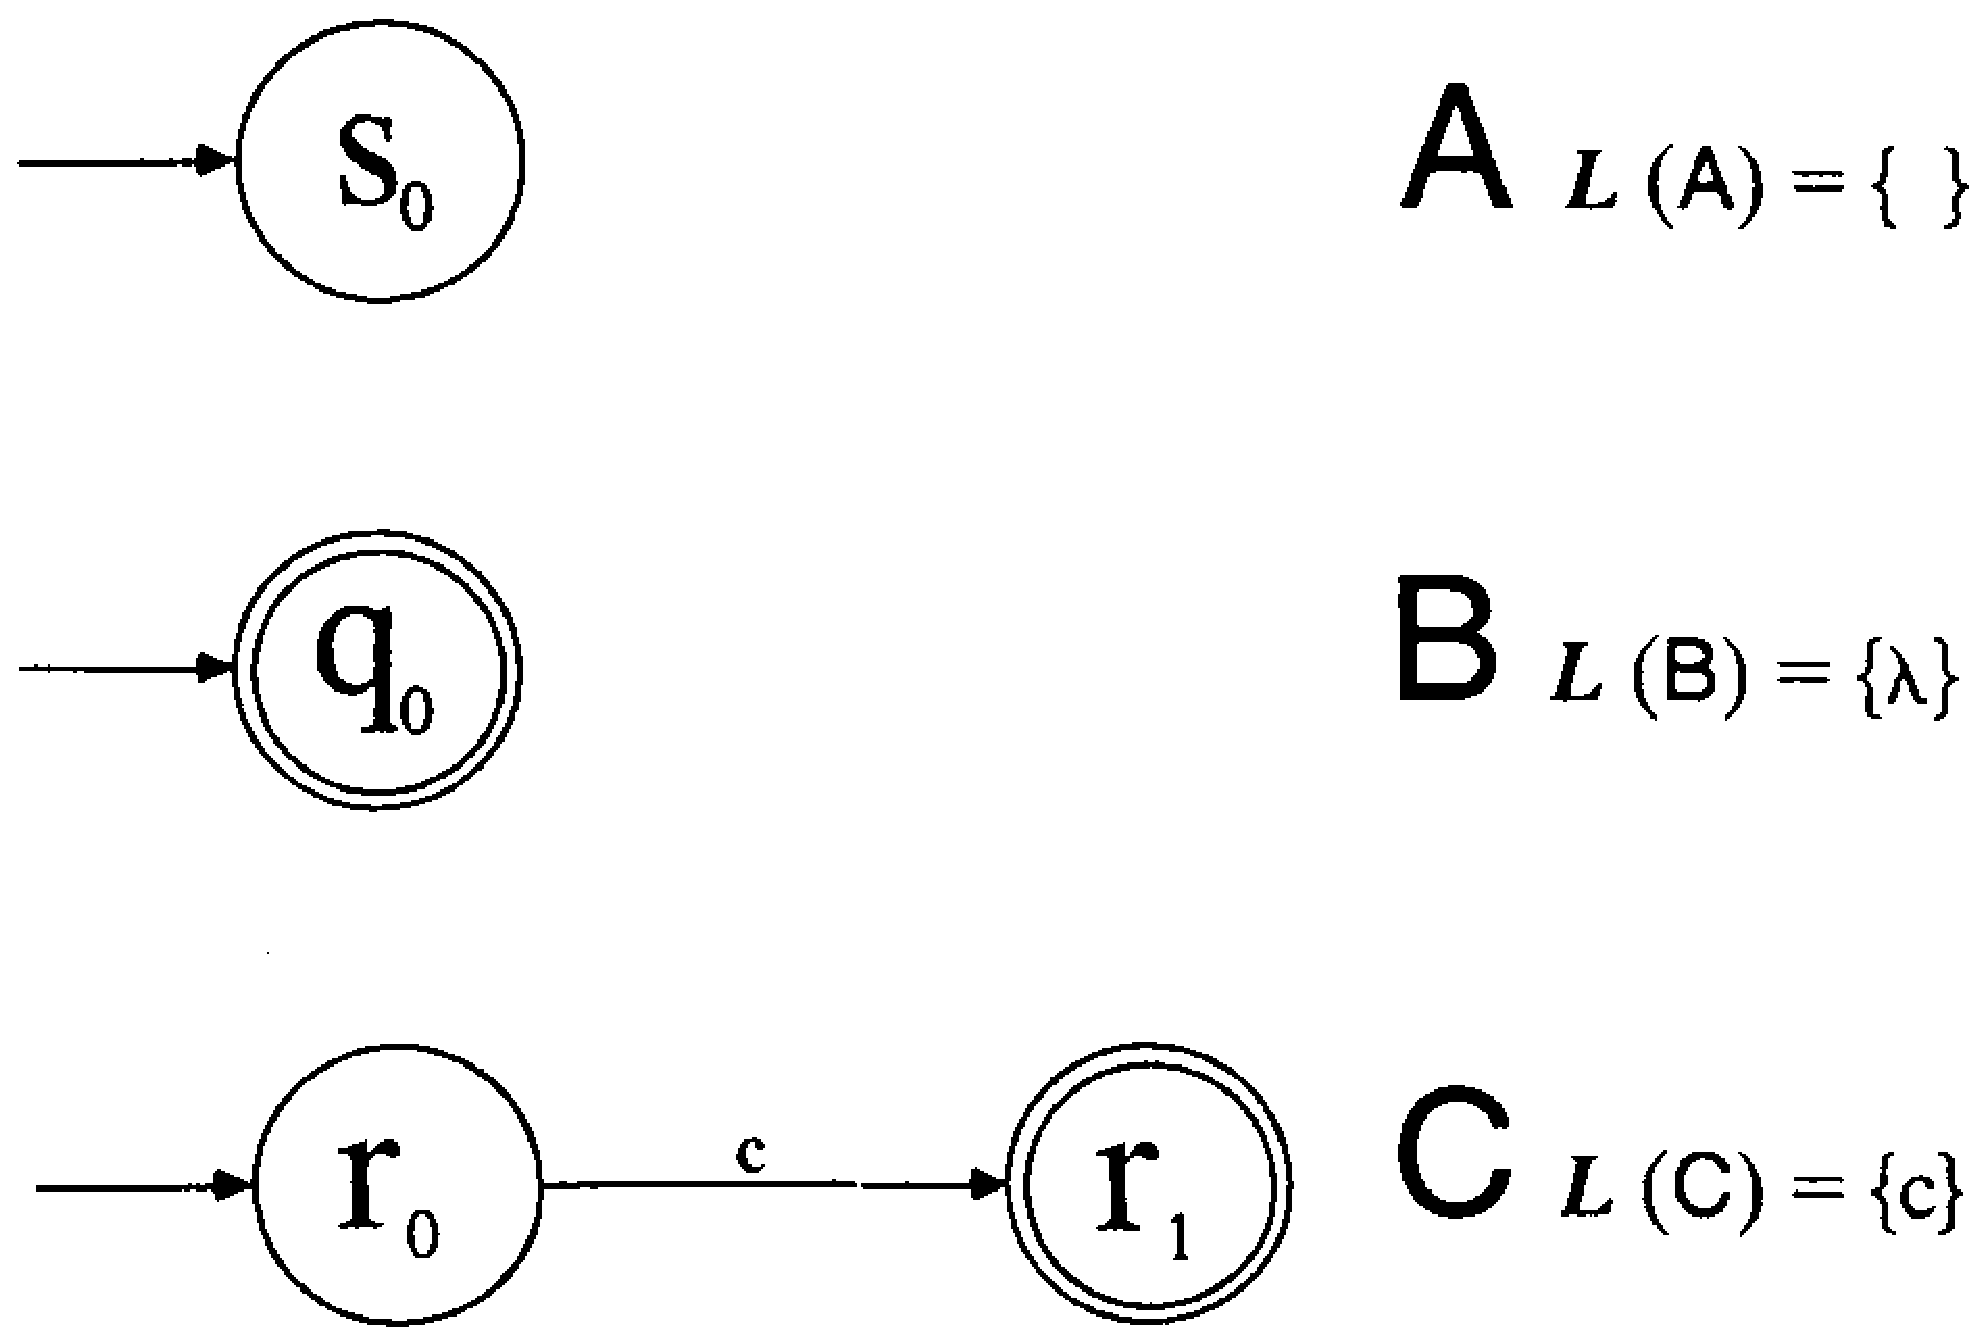
\epsfig{figure=ToFAfigures/fig6-1.eps,width=4in}}
\caption{NDFAs which recognize regular expressions with zero operators}\label{fig-6.1}
\end{figure}

% Figure 6.2
\begin{figure}
\centerline{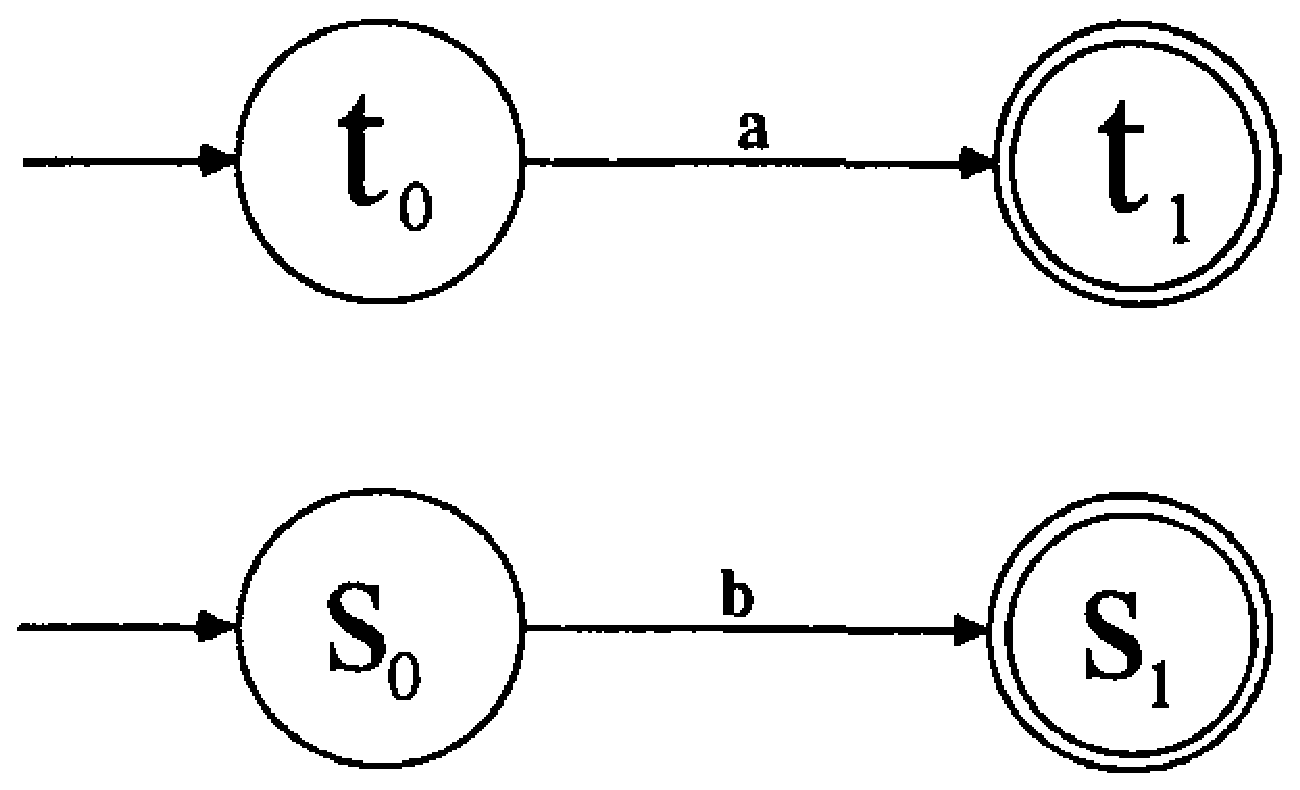
\epsfig{figure=ToFAfigures/fig6-2.eps,width=2.5in}}
\caption{The NDFA discussed in Example 6.4}\label{fig-6.2}
\end{figure}

\subsection*{Example 6.5}

An NDFA that accepts $(\pmb{a}\cup\pmb{b})^*$ is shown in Figure \ref{fig-6.3}. The
automaton given in Figure \ref{fig-6.2} for $(\pmb{a}\cup\pmb{b})$ is modified as
suggested by the proof of Theorem \ref{thm-5.5} to produce the \Index{Kleene closure} of
$(\pmb{a}\cup\pmb{b})$. Recall that the ``extra'' state $q_0$ was added to
ensure that $\lambda$ is accepted by the new machine.

% Figure 6.3
\begin{figure}
\centerline{\epsfig{figure=ToFAfigures/fig6-3.eps,width=2.5in}}
\caption{The NDFA discussed in Example 6.5}\label{fig-6.3}
\end{figure}

\subsection*{Example 6.6}

An NDFA that accepts $\pmb{c}\cdot(\pmb{a}\cup\pmb{b})^*$ (as suggested by the
proof of Theorem \ref{thm-5.4}) is shown in Figure \ref{fig-6.4}.

% Figure 6.4
\begin{figure}
\centerline{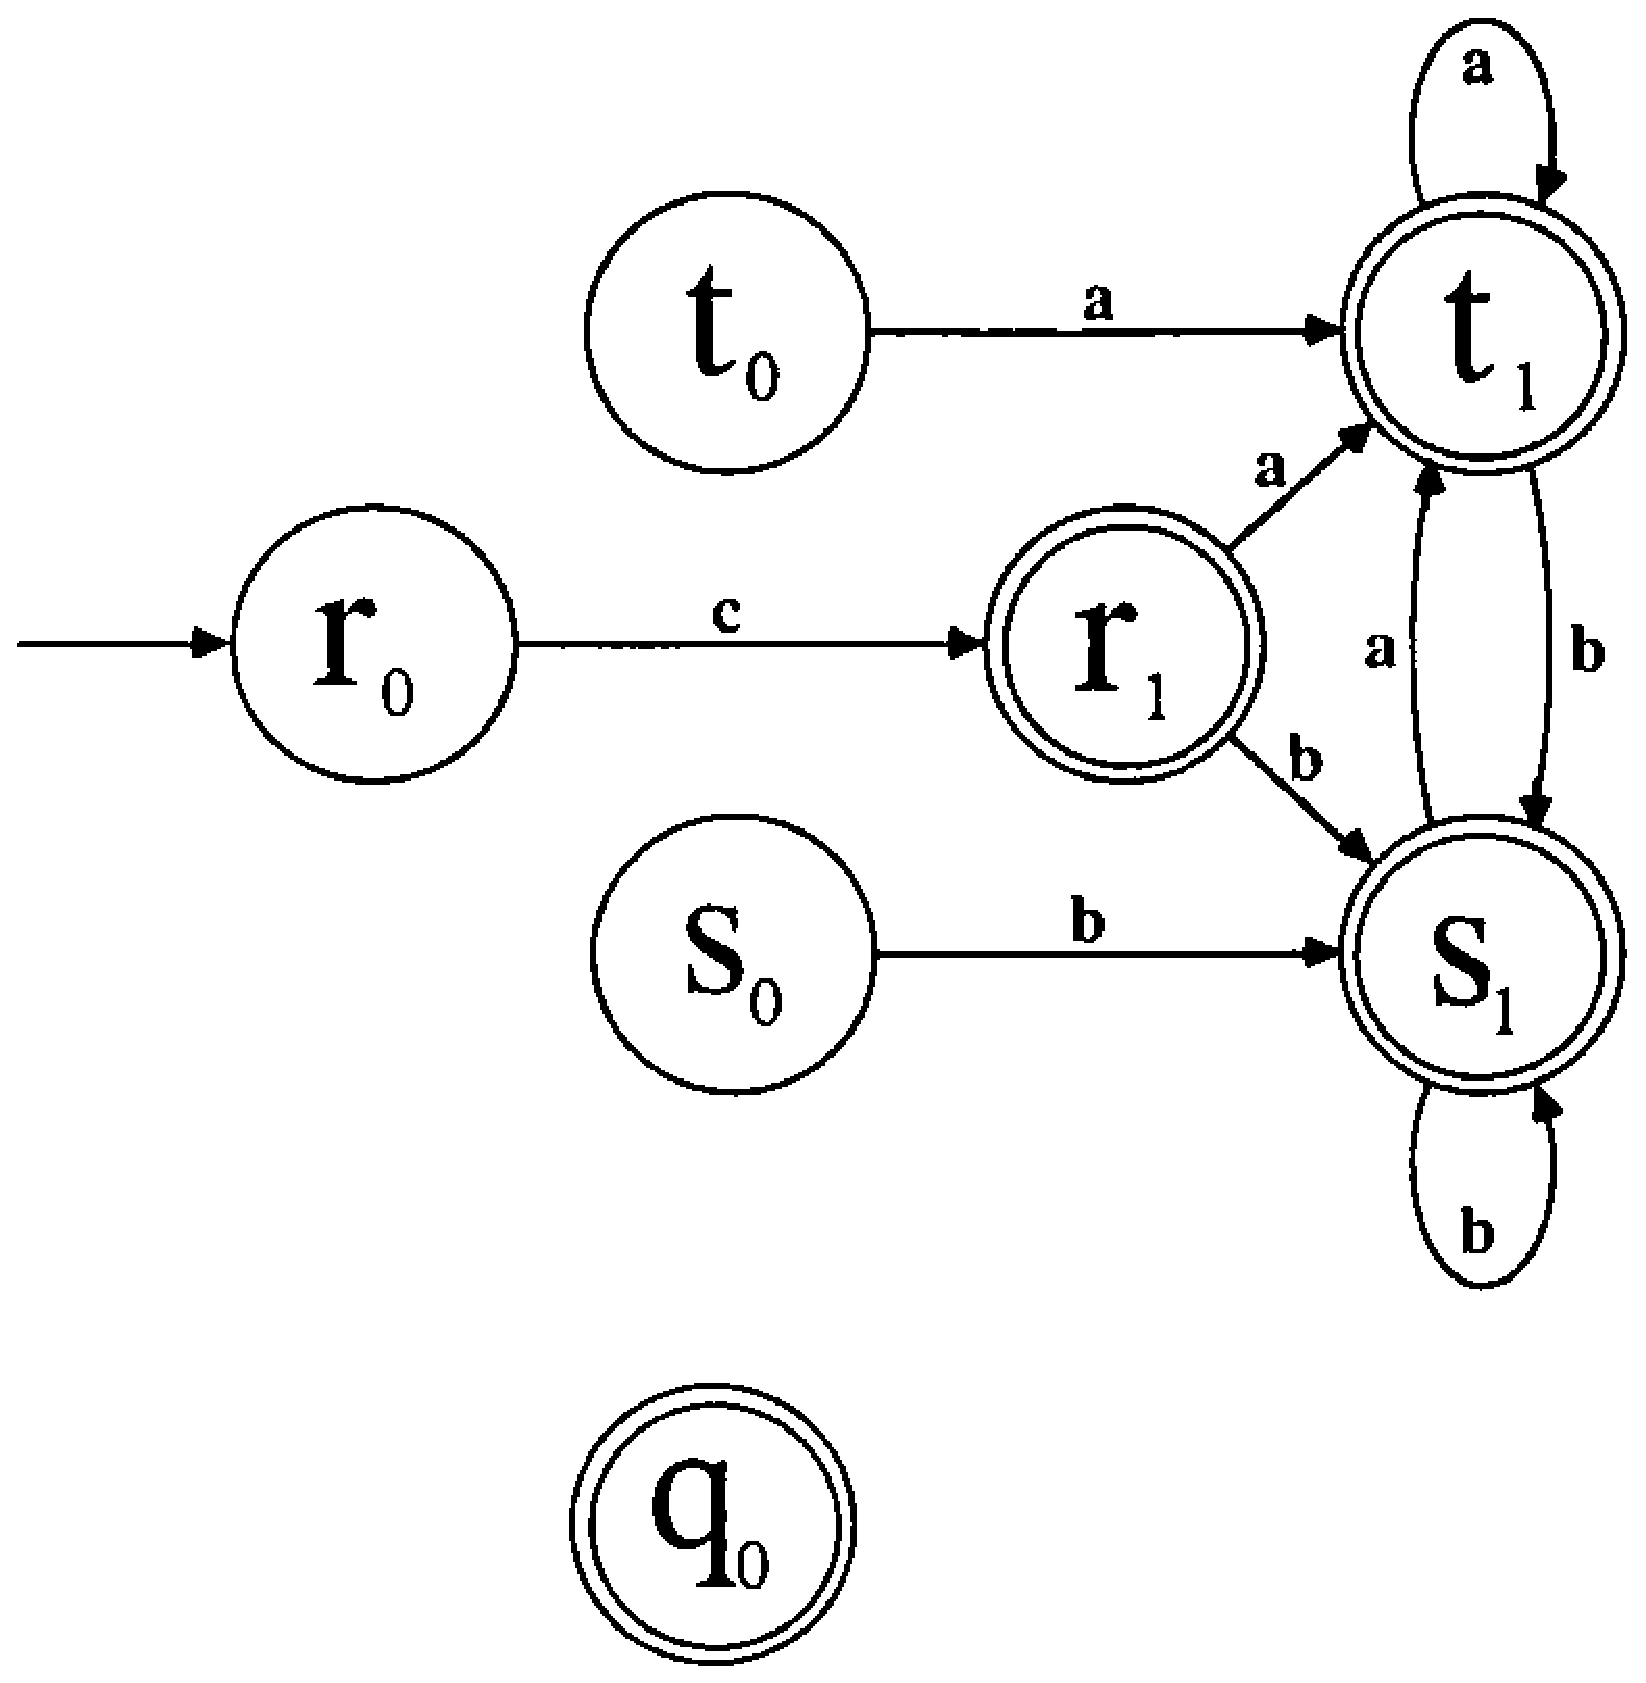
\epsfig{figure=ToFAfigures/fig6-4.eps,width=3.5in}}
\caption{The NDFA discussed in Example 6.6}\label{fig-6.4}
\end{figure}

Note that in this last example $q_0$, $t_0$, and $s_0$ are disconnected states,
and $r_1$, $s_1$, and $t_1$ could be coalesced into a single state. The
resulting machines are not advertised to be \emph{efficient}; the main point is that
they can be built. The techniques illustrated above are used to prove the
following lemma.

% Lemma 6.2
\begin{lmm}\label{lmm-6.2}
Let $\Sigma$ be an alphabet and let $R$ be a regular set over $\Sigma$. Then
there is a DFA that accepts $R$.

\emph{Proof.} The proof is by induction on the number of operators in the
regular expression describing $R$ (see the exercises). Note that Figure \ref{fig-6.1}
effectively illustrates the basis step: Those regular expressions with
\emph{zero} operators ($\emptyset,\epsilon,\pmb{a}_1,\pmb{a}_2,\ldots,\pmb{a}_m$)
do indeed correspond to FAD languages. This covers sets generated by rules i,
ii, and iii of Definition \ref{dfn-6.2}. For sets corresponding to regular expressions
with a positive number of operators, the outermost operator can be identified,
and it will be either $\cdot$, $\cup$, or $^*$, corresponding to an application
of rule iv, v, or vi. The induction assumption will guarantee that the
subexpressions used by the outermost operator have corresponding DFAs. Theorems
\ref{thm-5.2}, \ref{thm-5.4}, and \ref{thm-5.5} can then be invoked to argue that the entire expression has a
corresponding DFA.
\end{lmm}

% Corollary 6.1
\begin{cor}\label{cor-6.1}
Let $\Sigma$ be an alphabet. Then $\RSIG \subseteq \DSIG$.

\emph{Proof.} The proof follows immediately from Lemma \ref{lmm-6.2}.
\end{cor}

Since we are assured that every regular set can be accepted by a finite
automaton, the collection of regular sets is clearly contained in the set of FAD
languages. This also means that those languages that cannot be represented by a
DFA (that is, those contained in \NSIG) have no chance of being represented by a
regular expression.

\section{Language Equations}\label{sec-6.3}

The next question we will address is whether $\DSIG \subseteq \RSIG$, that is,
whether every FAD language can be represented by a regular expression. The
reader is invited to take a sample DFA and try to express the language it
accepts by a regular expression. You will probably be able to do it, but only by
guesswork and trial and error. Our first question appears to have a much more
methodical solution: Given a regular expression, it was a relatively
straightforward task to draw a NDFA (and then a DFA); in fact, we have a set of
\emph{algorithms} for doing just that, and we could program a computer to do the
task for us. This second question does not seem to have an obvious algorithm
connected with it, and we will have to attack the problem using a new concept:
\emph{\Index{language equations}}.

In algebra, we are used to algebraic equations such as $3x + 7 = 19$. Recall
that a \emph{solution} to this equation is a numerical value for $x$ that will make the
equation \emph{true}, that is, make both sides equal. In the above example, there is
only one choice for $x$, the unique solution 4. Equations can have two different
solutions, like $x^2=9$, no [real] solutions, like $x^2=-9$, or an \emph{infinite}
number of solutions, like $2(x+3) = x + 6 + x$. In a similar way, set equations
can be solved, such as $\{\pmb{a},\pmb{b},\pmb{c}\}=\{\pmb{a},\pmb{b}\}\cup X$.
Here $X$ represents a \emph{set}, and we are again looking for a value for $X$ that
will make the equation true; an obvious choice is $X=\{\pmb{c}\}$, but there are
other choices, like $X=\{\pmb{b},\pmb{c}\}$ (since $\{\pmb{a},\pmb{b},\pmb{c}\}=
\{\pmb{a},\pmb{b}\}\cup\{\pmb{b},\pmb{c}\})$. Such equations may likewise have
no solutions, like $X\cup\{\pmb{b}\}=\{\pmb{a},\pmb{c}\}$, or an infinite number
of solutions, such as $X\cup\{\pmb{b}\}=X$ (what sorts of sets satisfy this last
equation?). We wish to look at set equations where the sets are actually sets of
strings, that is, \emph{language} equations. The type of equation in which we
are most interested has one and only one solution, as outlined in the next
theorem. It is very similar in form and spirit to the theorem in algebra that
says ``For any numbers $a$ and $b$, where $a \not= 0$, the equation $ax=b$ has a
unique solution given by $x=b \div a$.''

% Theorem 6.1
\begin{thm}\label{thm-6.1}
Let $\Sigma$ be an alphabet. Let $E$ and $A$ be any subsets of $\Sigma^*$. Then
the language equation $X = E \cup A \cdot X$ admits the solution $X=A^*\!\!\cdot E$.
Any other solution $Y$ must contain $A^*\!\!\cdot E$.
Furthermore, if  $\lambda \notin A$, $X = A^*\!\!\cdot E$ is the unique solution.

\emph{Proof.} First note that the set $A^*E$ is indeed a solution to this
equation, since $A^*E = E \cup A \cdot (A^*E)$ (see the exercises). Now assume
that some set $Y$ is a solution to this equation, and let us investigate some of
the properties that $Y$ must have: If $Y$ is a solution, then
\begin{center}\begin{tabular}{rcl}
$Y = E \cup A \cdot Y$ & $\Rightarrow$ & (by definition of $\cup$) \\
$E \subseteq Y \wedge A \cdot Y \subseteq Y$ & $\Rightarrow$ &
	(if $E \subseteq Y$, then $A \cdot E \subseteq A \cdot Y$) \\
$A \cdot E \subseteq A \cdot Y \subseteq Y$ & $\Rightarrow$ & (by substitution) \\
$A \cdot A \cdot E \subseteq A \cdot A \cdot Y \subseteq A \cdot Y \subseteq Y$
	& $\Rightarrow$ & (by induction) \\
$(\forall n \in \NN)(A^n \cdot E \subseteq Y)$ & $\Rightarrow$ & (by definition
	of $A^*$) \\
$A^*\!\!\cdot E \subseteq Y$ &&
\end{tabular}\end{center}

Thus, every solution must contain all of $A^*E$, and $A^*E$ is in this sense the
smallest solution. This is true regardless of whether or not $\lambda$ belongs
to $A$.

Now let us assume that $\lambda \notin A$ and that we have a solution $W$ that
is actually ``bigger'' than $A^*E$; we will show that this is a contradiction,
and thus all solutions must look \emph{exactly} like $A^*E$. If $W$ is a
solution, $W \not= A^*E$, then there must be some elements in the set $W-A^*E$;
choose a string of \emph{minimal length} from among these elements and call it
$z$. Thus $z \in W$ and $z \notin A^*E$, and since $E \subseteq A^*E$ (why?),
$z \notin E$. Since $W$ is a solution, we have
\begin{center}\begin{tabular}{rcl}
$W=E \cup A \cdot W$ & $\Rightarrow$ & (since $z \in W$ and it cannot be in the
	$E$ part) \\
$z \in A \cdot W$ & $\Rightarrow$ & (by definition of $\cdot$) \\
$(\exists x \in A,\exists y \in W) \ni z = x \cdot y$ & $\Rightarrow$ & (by
	definition of $|\ |$) \\
$|z| = |x| + |y|$ & $\Rightarrow$ & (since $\lambda \notin A$ and $x \in A$, so
	$x \neq \lambda$ and $|x| > 0$) \\
|y| < |z|
\end{tabular}\end{center}

Note that $y$ cannot belong to $A^*E$ (if $y \in A^*E$, then, since $x \in A$,
$z(=x\cdot y)\in A \cdot (A^*E) \subseteq A^*E$, which means that $z \in A^*E$,
and we started by assuming that $z \notin A^*E$); since $y \in W$, we have 
$y \in W - A^*E$, and we have produced a string shorter than $z$, which belongs
to $W - A^*E$. This is the contradiction we were looking for, and we can
conclude that it is impossible for a solution $W$ to be larger than $A^*E$.
Since we have already shown that no solution can be smaller than $A^*E$, we now
know that the only solution is \emph{exactly} $A^*E$.
\end{thm}

\subsection*{Example 6.7}

$X=\{\pmb{b},\pmb{c}\} \cup \{\pmb{a}\} \cdot X$ does indeed have a solution;
$X$ can equal $\{\pmb{a}\}^*\!\!\cdot \{\pmb{b},\pmb{c}\}$. Note also that this is
the only solution (verify, for example, that $X=\{\pmb{a}\}^*\!\!\cdot\{\pmb{c}\}$
is \emph{not} a solution). The equation $Z=\{\pmb{b},\pmb{c}\}\cup\{\pmb{a},\lambda\}
\cdot Z$ has several solutions; among them are $Z=\{\pmb{a}\}^*\!\!\cdot\{\pmb{b},
\pmb{c}\}$ and $Z=\{\pmb{a},\pmb{b},\pmb{c}\}^*$.

It is instructive to explicitly list the first few elements of $\{\pmb{a}\}^*
\!\!\cdot\{\pmb{b},\pmb{c}\}$ and begin to check the validity of the solution to the
first equation. If $Y$ is a solution, then the two sides of the equation
$Y=\{\pmb{b},\pmb{c}\}\cup\{\pmb{a}\}\cdot Y$ must be equal. Since both $\pmb{b}$
and $\pmb{c}$ appear on the right-hand side they must also be on the left-hand
side, which clearly means that they have to be in $Y$. Once $\pmb{b}$ is known to
be in $Y$, it will give rise to a term on the right-hand side due to the
presence of $\{\pmb{a}\}\cdot Y$. Thus, $\pmb{a}\cdot\pmb{b}$ must also be found
on the left-hand side and therefore is in $Y$, and so on. The resulting sequence
of implications parallels the first part of the proof of Theorem \ref{thm-6.1}.

To see intuitively why no string other than those found in $\{\pmb{a}\}^*\cdot
\{\pmb{b},\pmb{c}\}$ may belong to a solution for $X=\{\pmb{b},\pmb{c}\}\cup\{
\pmb{a}\}\cdot X$, consider a string such as $\pmb{aa}$. If this were to belong to
$X$, then it would appear on the left-hand side and therefore would have to
appear on the right-hand side as well if the two sides were to indeed be equal.
On the right-hand side are just the two components, $\{\pmb{b},\pmb{c}\}$ and
$\{\pmb{a}\}\cdot X$. $\pmb{aa}$ is clearly not in $\{\pmb{b},\pmb{c}\}$, so it
must be in $\{\pmb{a}\}\cdot X$, which does seem plausible; all that is
necessary is for $\pmb{a}$ to be in $X$, and then \pmb{aa} will belong to $\{\pmb{a}\}
\cdot X$. If $\pmb{a}$ is in $X$, though, it must also appear on the left-hand
side, and so $\pmb{a}$ must be on the right-hand side as well. Again, $\pmb{a}$ is
not in $\{\pmb{b},\pmb{c}\}$, so it must be in $\{\pmb{a}\}\cdot X$. This can
happen only if $\lambda$ belongs to $X$ so that $\pmb{a}\cdot\lambda$ will
belong to $\{\pmb{a}\}\cdot X$. This implies that $\lambda$ must now show up on
both sides, and this leads to a contradiction: $\lambda$ cannot be on the
right-hand side since $\lambda$ clearly is not in $\{\pmb{b},\pmb{c}\}$, and it
cannot belong to $\{\pmb{a}\}\cdot X$ either, since all these words begin with
an $\pmb{a}$. This contradiction shows why $\pmb{aa}$ cannot be part of any solution
$X$.

This example illustrates the basic nature of these types of equations: for words
that are not in $\{\pmb{a}\}^*\!\!\cdot\{\pmb{b},\pmb{c}\}$, the inclusion of that
word in the solution leads to the inclusion of shorter and shorter strings,
which eventually leads to a contradiction. This property was exploited in the
second half of the proof of Theorem \ref{thm-6.1}. Rather than finding shorter and shorter
strings, though, it was assumed we already had the shortest, and we showed that
there had to be a still shorter one; this led to the desired contradiction more
directly.

Our main goal will be to solve \emph{systems} of language equations, since the
relationships between the \emph{terminal sets} of an automaton can be described
by such a system. Systems of language equations are similar in form and spirit
to systems of algebraic equations, such as
\begin{center}\begin{tabular}{c}
$3x_1 + x_2 = 10$ \\
$x_1 - x_2 = 2$
\end{tabular}\end{center}
which has the unique solution $x_1 = 3$, $x_2 = 1$. We will look at systems of
language equations such as
\begin{center}\begin{tabular}{l}
$X_1 = \epsilon \cup \pmb{a} \cdot X_1 \cup \pmb{b} \cdot X_2$ \\
$X_2 = \emptyset \cup \pmb{b} \cdot X_1 \cup \emptyset \cdot X_2$
\end{tabular}\end{center}
which has the (unique) solution $X_1=(\pmb{a}\cup\pmb{bb})^*,X_2=\pmb{b}\cdot(
\pmb{a}\cup\pmb{bb})^*$. Checking that this is a solution entails verifying that
both equations are satisfied if these expressions are substituted for the
variables $X_1$ and $X_2$.

The solution of such systems parallels the solution of algebraic equations.
For example, the system
\begin{center}\begin{tabular}{c}
$3x_1 + x_2 = 10$ \\
$x_1 - x_2 = 2$
\end{tabular}\end{center}
can be solved by treating the second statement as an equation in just the
variable $x_2$ and solving as indicated by the algebraic theorem ``For any
numbers $a$ and $b$, where $a \not= 0$, the equation $ax = b$ has a unique
solution given by $x = b \div a$.'' The second statement can be written as
$(-1)x_2 = 2 - x_1$, which then admits the solution $x_2=(2-x_1)\div(-1)$ or
$x_2=x_1-2$. This solution can be inserted into the first equation to eliminate
$x_2$ and form an equation solely in $x_1$. Terms can be regrouped and the
algebraic theorem can be applied to find $x_1$. We would have
\[ 3x_1 + x_2 = 10 \]
which becomes
\[ 3x_1 + x_1 - 2 = 10 \]
or
\[ 4x_1 - 2 = 10 \]
or
\[ 4x_1 = 12 \]
or
\[ x_1 = 12 \div 4 \]
yielding
\[ x_1 = 3 \]
This value of $x_1$ can be back-substituted to find the unique solution for
$x_2$: $x_2=x_1-2=3-2=1$.

Essentially, the same technique can be applied to any two equations in two
unknowns, and formulas can be developed that predict the coefficients for the
reduced set of equations. Consider the generalized system of algebraic equations
with unknowns $x_1$ and $x_2$, constant terms $E_1$ and $E_2$, and coefficients
$A_{11},\ A_{12},\ A_{21},$ and $A_{22}$:
\begin{center}\begin{tabular}{c}
$A_{11}x_1 + A_{12}x_2 = E_1$ \\
$A_{21}x_1 + A_{22}x_2 = E_2$
\end{tabular}\end{center}
Recall that the appropriate formulas for reducing this to a single equation of
the form $\hat{A}_{11}x_1 = \hat{E}_1$, where the new coefficients
$\hat{A}_{11}$ and $\hat{E}_1$ can be calculated as
\begin{center}\begin{tabular}{c}
$\hat{E}_1 = E_1A_{22} - E_2A_{12}$ \\
$\hat{A}_{11} = A_{11}A_{22} - A_{12}A_{21}$
\end{tabular}\end{center}
A similar technique can be used to eliminate variables when there is a larger
number of equations in the system. The following theorem makes similar
predictions of the new coefficients for language equations.

% Theorem 6.2
\begin{thm}\label{thm-6.2}
Let $n \geq 2$ and consider the system of equations in the unknowns $X_1,X_2,
\ldots,X_n$ given by
\begin{center}\begin{tabular}{rcl}
$X_1$ & $=$ & $E_1 \cup A_{11}X_1 \cup A_{12}X_2 \cup \cdots \cup A_{1(n-1)}
	X_{n-1} \cup A_{1n}X_n$ \\
$X_2$ & $=$ & $E_2 \cup A_{21}X_1 \cup A_{22}X_2 \cup \cdots \cup A_{2(n-1)}
	X_{n-1} \cup A_{2n}X_n$ \\
$\cdot$ && \\
$\cdot$ && \\
$\cdot$ && \\
$X_{n-1}$ & $=$ & $E_{n-1} \cup A_{(n-1)1}X_1 \cup A_{(n-1)2}X_2 \cup \cdots
	\cup A_{(n-1)(n-1)}X_{n-1} \cup A_{(n-1)n}X_n$ \\
$X_n$ & $=$ & $E_n \cup A_{n1}X_1 \cup A_{n2}X_2 \cup \cdots \cup
	A_{n(n-1)}X_{n-1} \cup A_{nn}X_n$
\end{tabular}\end{center}
in which $(\forall i,j \in \{1,2, \cdots ,n\})(\lambda \notin A_{ij})$.
\begin{enumerate}[a.]
\item This system has a unique solution.
\item Define $\hat{E}_i = E_i \cup (A_{in} \cdot A^*_{nn} \cdot E_n)$ for all
	$i=1,2, \cdots ,n - 1$ \\
and
\[ \hat{A}_{ij} = A_{ij} \cup (A_{in} \cdot A^*_{nn} \cdot A_{nj})\text{ for
	all }i,j = 1,2, \cdots ,n - 1. \]
The solution to the original set of equations will agree with the solution to
the following set of $n-1$ equations in the unknowns $X_1,X_2,\cdots,X_{n-1}$:
\begin{center}\begin{tabular}{rcl}
$X_1$ & $=$ & $\hat{E}_1 \cup \hat{A}_{11}X_1 \cup \hat{A}_{12}X_2 \cup \cdots
	\cup \hat{A}_{1(n-1)}X_{n-1}$ \\
$X_2$ & $=$ & $\hat{E}_2 \cup \hat{A}_{21}X_1 \cup \hat{A}_{22}X_2 \cup \cdots
	\cup \hat{A}_{2(n-2)}X_{n-1}$ \\
$\cdot$ && \\
$\cdot$ && \\
$\cdot$ && \\
$X_{n-1}$ & $=$ & $\hat{E}_{n-1} \cup \hat{A}_{(n-1)1}X_1 \cup \hat{A}_{(n-1)2}
	X_2 \cup \cdots \cup \hat{A}_{(n-1)(n-1)}X_{n-1}$
\end{tabular}\end{center}
\item Once the solution to the above $n - 1$ equations in (b) is known, that
solution can be used to find the remaining unknown:
\[ X_n = A^*_{nn} \cdot (E_n \cup A_{n1}X_1 \cup A_{n2}X_2 \cup \cdots \cup
	A_{n(n-1)}X_{n-1}) \]
\end{enumerate}

\emph{Proof.} The proof hinges on the repeated application of Theorem \ref{thm-6.1}. The
last of the $n$ equations, $X_n = E_n \cup A_{n1}X_1 \cup A_{n2}X_2 \cup \cdots
\cup A_{n(n-1)}X_{n-1} \cup A_{nn}X_{n}$ can be thought of as an equation in the
one unknown $X_n$ with a coefficient of $A_{nn}$ for $X_n$, and the remainder of
the expression a ``constant'' term not involving $X_n$. The following
parenthetical grouping illustrates this viewpoint:
\[ X_n = (E_n \cup A_{n1}X_1 \cup A_{n2}X_2 \cup \cdots \cup A_{n(n-1)}X_{n-1})
	\cup A_{nn}X_n \]
Note that for any subscript $k$, if $A_{nk}$ does not contain $\lambda$, neither
will $A_{nk}X_k$. Theorem \ref{thm-6.1} can therefore be applied, to the one equation in
the one unknown $X_n$, with coefficients
\[ E = (E_n \cup A_{n1}X_1 \cup A_{n2}X_2 \cup \cdots \cup A_{n(n-1)}X_{n-1}) \]
and $A = A_{nn}$. The solution, $A^*E$, is exactly as given by part (c) above:
\[ X_n = A^*_{nn} \cdot (E_n \cup A_{n1}X_1 \cup A_{n2}X_2 \cup \cdots \cup
	A_{n(n-1)}X_{n-1}) \]
or
\[ X_n = A^*_{nn} \cdot E_n \cup A^*_{nn} \cdot A_{n1}X_1 \cup A^*_{nn} \cdot
	A_{n2}X_2 \cup \cdots \cup A^*_{nn} \cdot A_{n(n-1)}X_{n-1} \]
If there was a unique solution for the terms $X_1$ through $X_{n-1}$, then
Theorem \ref{thm-6.1} would guarantee a unique solution for $X_n$, too.

The solution for $X_n$ can be substituted for $X_n$ in each of the other $n-1$
equations. If the $k$th equation is represented by
\[ X_k = E_k \cup A_{k1}X_1 \cup A_{k2}X_2 \cup \cdots \cup A_{kn}X_n \]
then the substitution will yield \\
\begin{tabular}{lll}
$X_k$ & $=$ & $E_k \cup A_{k1}X_1 \cup A_{k2}X_2 \cup \cdots$ \\
&& $\cup (A_{kn} \cdot (A^*_{nn} \cdot E_n \cup A^*_{nn} \cdot A_{n1}X_1 \cup
	A^*_{nn} \cdot A_{n2}X_2 \cup \cdots \cup A^*_{nn} \cdot
	A_{n(n-1)}X_{n-1}))$
\end{tabular} \\
By using the distributive law, this becomes \\
\begin{tabular}{lll}
$X_k$ & $=$ & $E_k \cup A_{k1}X_1 \cup A_{k2}X_2 \cup \cdots$ \\
&& $\cup (A_{kn} \cdot A^*_{nn} \cdot E_n \cup A_{kn} \cdot A^*_{nn} \cdot
	A_{n1}X_1 \cup A_{kn} \cdot A^*_{nn} \cdot A_{n2}X_2 \cup \cdots \cup
	A_{kn} \cdot A^*_{nn} \cdot A_{n(n-1)}X_{n-1})$
\end{tabular} \\
Collecting like terms yields \\
\begin{tabular}{lll}
$X_k$ & $=$ & $(E_k \cup A_{kn} \cdot A^*_{nn} \cdot E_n) \cup (A_{k1}X_1 \cup
	A_{kn} \cdot A^*_{nn} \cdot A_{n1}X_1)$ \\
&& $\cup (A_{k2}X_2 \cup A_{kn} \cdot A^*_{nn} \cdot A_{n2}X_2) \cup \cdots \cup
	(A_{k(n-1)}X_{n-1} \cup A_{kn} \cdot A^*_{nn} \cdot A_{n(n-1)}X_{n-1})$
\end{tabular} \\
or
\begin{center}\begin{tabular}{l}
$X_k = (E_k \cup A_{kn} \cdot A^*_{nn} \cdot E_n) \cup (A_{k1} \cup A_{kn}
	\cdot A^*_{nn} \cdot A_{n1})X_1$ \\
$\qquad \cup (A_{k2} \cup A_{kn} \cdot A^*_{nn} \cdot A_{n2})X_2 \cup \cdots
	\cup (A_{k(n-1)} \cup A_{kn} \cdot A^*_{nn} \cdot A_{n(n-1)})X_{n-1}$
\end{tabular}\end{center}
The constant term in this equation is $(E_k \cup A_{kn} \cdot A^*_{nn} \cdot
E_n)$, which is exactly the formula given for $\hat{E}_k$ in part (b). The
coefficient for $X_1$ is seen to be
\[ (A_{k1} \cup A_{kn} \cdot A^*_{nn} \cdot A_{n1}), \]
while the coefficient for $X_2$ is $(A_{k2} \cup A_{kn} \cdot A^*_{nn} \cdot
A_{n2})$, and so on. The coefficient for $X_j$ would then be $\hat{A}_{kj} =
A_{kj} \cup (A_{kn} \cdot A^*_{nn} \cdot A_{nj})$, which also agrees with the
formula given in part (b). This is why the solution of the original set of
equations agrees with the solution of the set of $n-1$ equations given in part
(b).

Part (a) is proved by induction on $n$: the method outlined above can be
repeated on the new set of $n-1$ equations to eliminate $X_{n-1}$ and so on,
until one equation in the one unknown $X_1$ is obtained. Theorem \ref{thm-6.1} will
guarantee a unique solution for $X_1$, and part (c) can then be used to find the
unique solution for $X_2$, and so on.
\end{thm}

\subsection*{Example 6.8}

Consider the system defined before, where
\begin{center}\begin{tabular}{r@{ = }l}
$X_1$ & $\epsilon \cup \pmb{a} \cdot X_1 \cup \pmb{b} \cdot X_2$ \\
$X_2$ & $\emptyset \cup \pmb{b} \cdot X_1 \cup \emptyset \cdot X_2$
\end{tabular}\end{center}
The proof of Theorem \ref{thm-6.2} implies the solution for $X_1$ will agree with the
solution to the one-variable equation $X_1 = \hat{E}_1 \cup \hat{A}_{11}X_1$,
where
\[ \hat{E}_1 = E_1 \cup (A_{12}\cdot A^*_{22}\cdot E_2) = \epsilon \cup (\pmb{b} \cdot \emptyset^*\!\!
	\cdot \emptyset) = \epsilon \cup (\pmb{b}\cdot\epsilon\cdot\emptyset) =
	\epsilon \cup \emptyset = \epsilon \]
and
\[ \hat{A}_{11} = A_{11} \cup (A_{12} \cdot A^*_{22} \cdot A_{21}) = \pmb{a}
	\cup (\pmb{b}\cdot\emptyset^*\!\!\cdot\pmb{b}) = \pmb{a} \cup (\pmb{b} \cdot
	\epsilon \cdot \pmb{b}) = \pmb{a} \cup \pmb{bb}. \]
Thus we have $X_1 = \epsilon \cup (\pmb{a} \cup \pmb{bb})\cdot X_1$, which by
Theorem \ref{thm-6.1} has the (unique) solution $X_1 = \hat{A}^*_{11}\hat{E}_1 = (\pmb{a}
\cup \pmb{bb})^*\!\! \cdot \epsilon$. Substituting this into the second equation
yields $X_2 = \emptyset \cup \pmb{b}\cdot(\pmb{a}\cup\pmb{bb})^*\cup\emptyset
\cdot X_2$, which by Theorem \ref{thm-6.1} has the (unique) solution $X_2=\emptyset^*\!\!\cdot
(\pmb{b}\cdot(\pmb{a}\cup\pmb{bb})^*) = \pmb{b} \cdot (\pmb{a}\cup\pmb{bb})^*$\!.
Note that this expression for $X_2$ could also be found by applying the
back-substitution formula given in the proof of Theorem \ref{thm-6.2}.

We will now see that the language accepted by a DFA can be equated with the
solution of a set of language equations, which will allow us to prove the
following important theorem.

% Theorem 6.3
\begin{thm}\label{thm-6.3}
Let $\Sigma$ be an alphabet and let $L$ be an FAD language over $\Sigma$. Then
$L$ is a regular set over $\Sigma$.

\emph{Proof.} If $L$ is FAD, then there exists an $n > 0$ and a deterministic
finite automaton $A=\langle\Sigma,\{s_1,s_2, \ldots,\\s_n\},s_1,\delta,F\rangle$
such that $L(A) = L$. For each $i = 1,2,\ldots ,n,$ define $X_i=\{z \in \Sigma^*
|\ \DBAR(s_i,z) \in F\}$; that is, $X_i$ is the set of all strings that, \emph{when
starting at state} $s_i$, reach a final state in $A$. Each $X_i$ then represents
the terminal set $T(A,s_i)$ described in Chapter \ref{ch-3}. Since $s_1$ is the start state
of this machine, it should be clear that $X_1 = L(A) = L$. Define
\begin{align*}
E_i = & \left\{ \begin{tabular}{ll}
			$\emptyset$ & if $s_i \notin F$ \\
			& \\
			$\epsilon$ & if $s_i \in F$
		 \end{tabular}\right. &
		 \text{for }i = 1,2,\ldots,n \\
\intertext{and}
A_{ij} = & \bigcup\limits_{\pmb{a}\,\in\,\Sigma\,\wedge\,\delta(s_i,\pmb{a})\,=\,
	s_j} \pmb{a} & \text{for }i,j=1,2, \ldots ,n
\end{align*}
That is, $A_{ij}$ represents the set of all letters that cause a transition from
state $s_i$ to state $s_j$. Notice that since $\lambda\notin\Sigma$ none of the
sets $A_{ij}$ contain the empty string, and therefore by Theorem \ref{thm-6.2}, there is a
unique solution to the system:
\begin{center}\begin{tabular}{rcl}
$X_1$ & $=$ & $E_1 \cup A_{11}X_1 \cup A_{12}X_2 \cup \cdots \cup A_{1n}X_n$ \\
$X_2$ & $=$ & $E_2 \cup A_{21}X_1 \cup A_{22}X_2 \cup \cdots \cup A_{2n}X_n$ \\
& $\cdot$ & \\ & $\cdot$ & \\ & $\cdot$ & \\
$X_n$ & $=$ & $E_n \cup A_{n1}X_1 \cup A_{n2}X_2 \cup \cdots \cup A_{nn}X_n$
\end{tabular}\end{center}
However, these equations exactly describe the relationships between the terminal
sets denoted by $X_1,X_2, \cdots ,\\X_n$, at the beginning of this proof (compare
with Example 6.11), and hence the solution will represent exactly those
quantities. In particular, the solution for $X_1$ will be a regular expression
for $L(A)$, that is, for $L$.
\end{thm}

\subsection*{Example 6.9}

Consider the DFA $B$ given by the diagram in Figure \ref{fig-6.5}, which accepts all
strings with an odd number of $\pmb{b}$s over $\{\pmb{a},\pmb{b}\}$. This machine
generates the following system of language equations:
\begin{align*}
& X_1 = \emptyset \cup \pmb{a}X_1 \cup \pmb{b}X_2 \\
& X_2 = \epsilon \cup \pmb{b}X_1 \cup \pmb{a}X_2
\end{align*}
which will have the same solution for $X_1$ as the equation
\[ X_1 = \hat{E}_1 \cup \hat{A}_{11}X_1 \]
where
\[ \hat{E}_1 = E_1 \cup (A_{12}\cdot A^*_{22}\cdot E_2) = \emptyset \cup
	(\pmb{b}\cdot\pmb{a}^*\cdot\epsilon) = \pmb{b}\cdot\pmb{a}^* \]
and
\[ \hat{A}_{11} = A_{11} \cup (A_{12}\cdot A^*_{22}\cdot A_{21}) = \pmb{a} \cup
	(\pmb{b}\cdot\pmb{a}^*\cdot\pmb{b}) \]
% Figure 6.5
\begin{figure}
\centerline{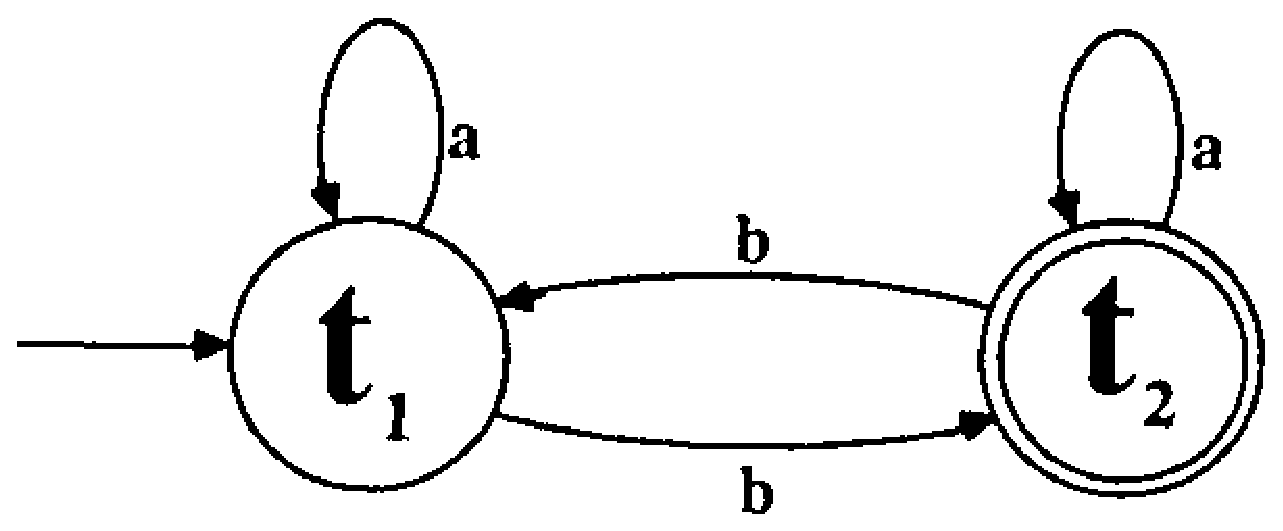
\epsfig{figure=ToFAfigures/fig6-5.eps,width=2.5in}}
\caption{The DFA discussed in Example 6.9}\label{fig-6.5}
\end{figure}
Theorem \ref{thm-6.1} predicts the solution for $X_1$ to be $(\pmb{a}\cup(\pmb{b}\cdot
\pmb{a}^*\cdot\pmb{b}))^*\cdot\pmb{b}\cdot\pmb{a}^*$. It can be verified that
this solution describes all those strings with an odd number of $\pmb{b}$s. $X_1$
is indeed the terminal set for $t_1$, that is, $T(B,t_1)$. Likewise, finding
$X_2$ yields all strings with an even number of $\pmb{b}$s, which is the terminal
set for $t_2$, $T(B,t_2)$.

Nondeterministic finite automata can likewise be represented by language
equations, and without the intermediate step of applying Definition \ref{dfn-4.5} to
acquire a deterministic equivalent. The sets $E_i$ and $A_{ij}$ retain
essentially the same definitions as before: $E_i$ is $\epsilon$ or $\emptyset$,
depending on whether or not $s_i$ is a final state, and $A_{ij}$ again
represents exactly the set of all letters that cause a transition from state
$s_i$ to state $s_j$. This definition requires a minor cosmetic change for
NDFAs, since the state transition function is slightly different:
\[ A_{ij} = \bigcup\limits_{\pmb{a}\,\in\,\Sigma\,\wedge\,s_j\,\in\,\delta(s_i,
	\pmb{a})}\pmb{a}\qquad\text{for }i,j=1,2, \ldots ,n \]

An $n$-state NDFA therefore gives rise to $n$ equations in $n$ unknowns, which
can be solved as outlined by Theorems \ref{thm-6.2} and \ref{thm-6.1}. While Definition \ref{dfn-4.5} need not
be used as a conversion step, an NDFA with $\lambda$-moves will have to be
transformed into an equivalent NDFA without $\lambda$-moves. An appropriate
definition for $A_{ij}$ \emph{could} be given for the original NDFA, and while
the resulting equations would describe the relation between the terminal sets,
some $A_{ij}$ set might then contain $\lambda$ as a member. There are systems of
equations arising in this manner that do not have unique solutions (see the
exercises). For an NDFA with $\lambda$-moves, Definition \ref{dfn-4.9} could be applied to
find an equivalent NDFA without $\lambda$-moves, since Theorems \ref{thm-6.2} and \ref{thm-6.1}
specifically prohibit the empty string as a part of a coefficient. However, if
the ambiguous equations generated from a machine with $\lambda$-moves were
solved as suggested in Theorems \ref{thm-6.1} and \ref{thm-6.2}, a ``minimal'' solution would be
obtained that would correspond to the desired answer.

\subsection*{Example 6.10}

Consider again the system described in Example 6.8. This can be thought of as
the set of language equations corresponding to the NDFA called $B$, illustrated
in Figure \ref{fig-6.6}a. Note that $L(B)$ is indeed the given solution: $L(B) = X_1 =
(\pmb{a}\cup\pmb{bb})^*$. Notice the similarity between $B$ and the machine $C$
shown in Figure \ref{fig-6.6}b, which has $s_2$ as the start state. Note that $L(C)$ is
given by $X_2=\pmb{b}\cdot(\pmb{a}\cup\pmb{bb})^*$, where $X_2$ was the other
part of the solution given in Example 6.8 (verify this). Finally, consider a
similar machine $D$ in Figure \ref{fig-6.6}c with both $s_1$ and $s_2$ as start states.
Can you quickly write a regular expression that describes the language accepted
by $D$?

% Figure 6.6
\begin{figure}
\centerline{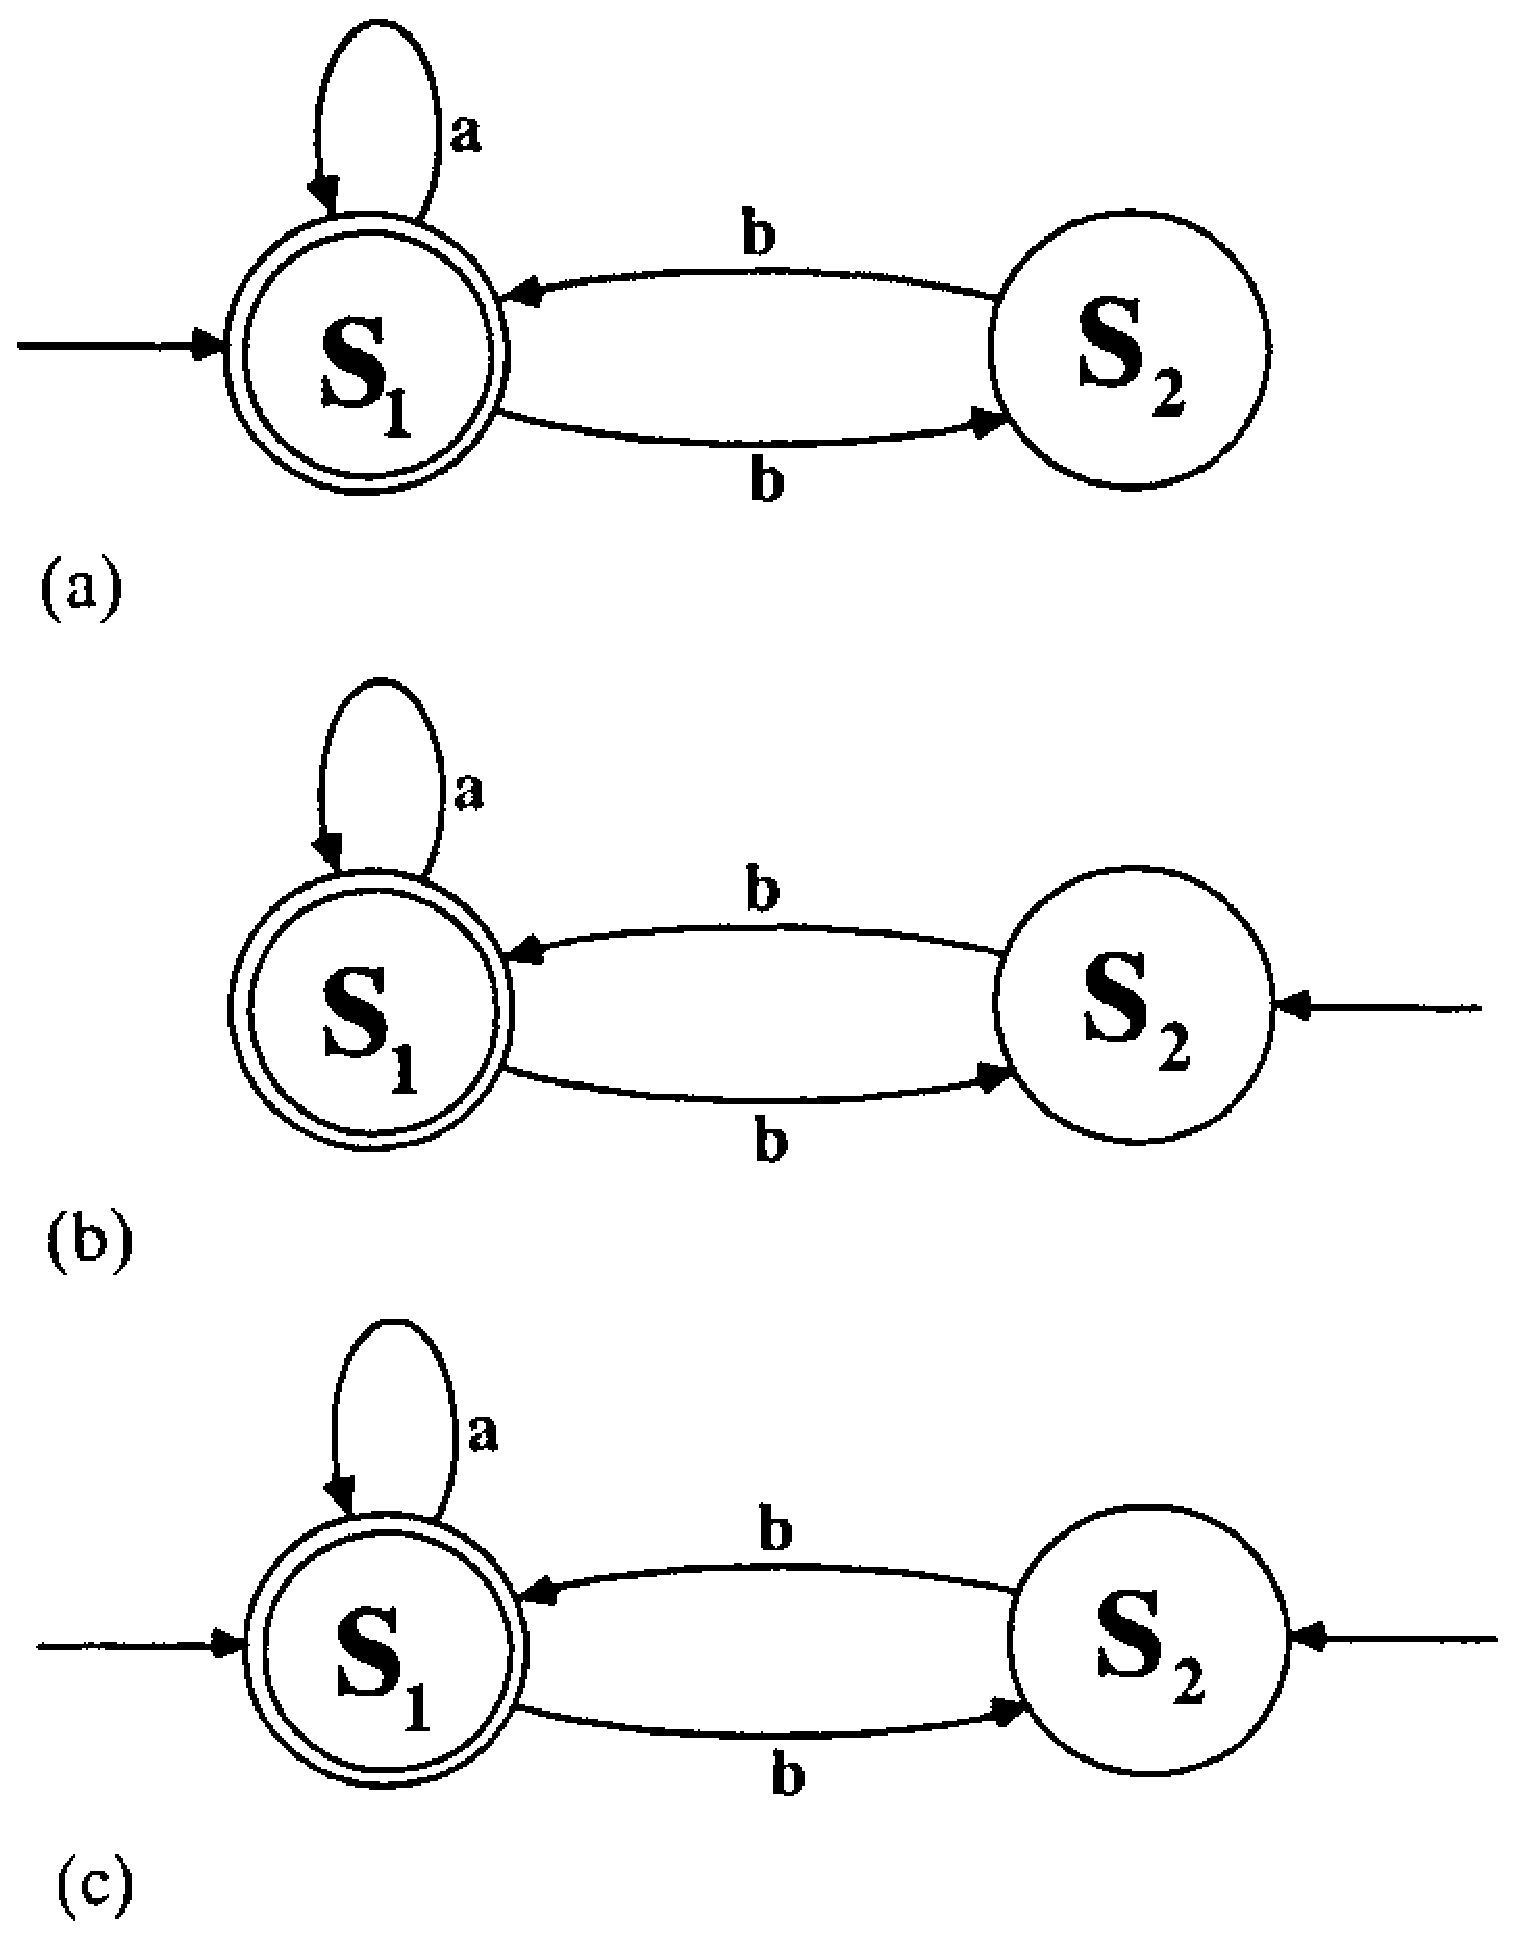
\epsfig{figure=ToFAfigures/fig6-6.eps,width=2.5in}}
\caption{(a) The NDFA $B$ discussed in Example 6.10 (b) The NDFA $C$
discussed in Example 6.10 (c) The NDFA $D$ discussed in Example 6.10}\label{fig-6.6}
\end{figure}

\subsection*{Example 6.11}

% Figure 6.7
\begin{figure}
\centerline{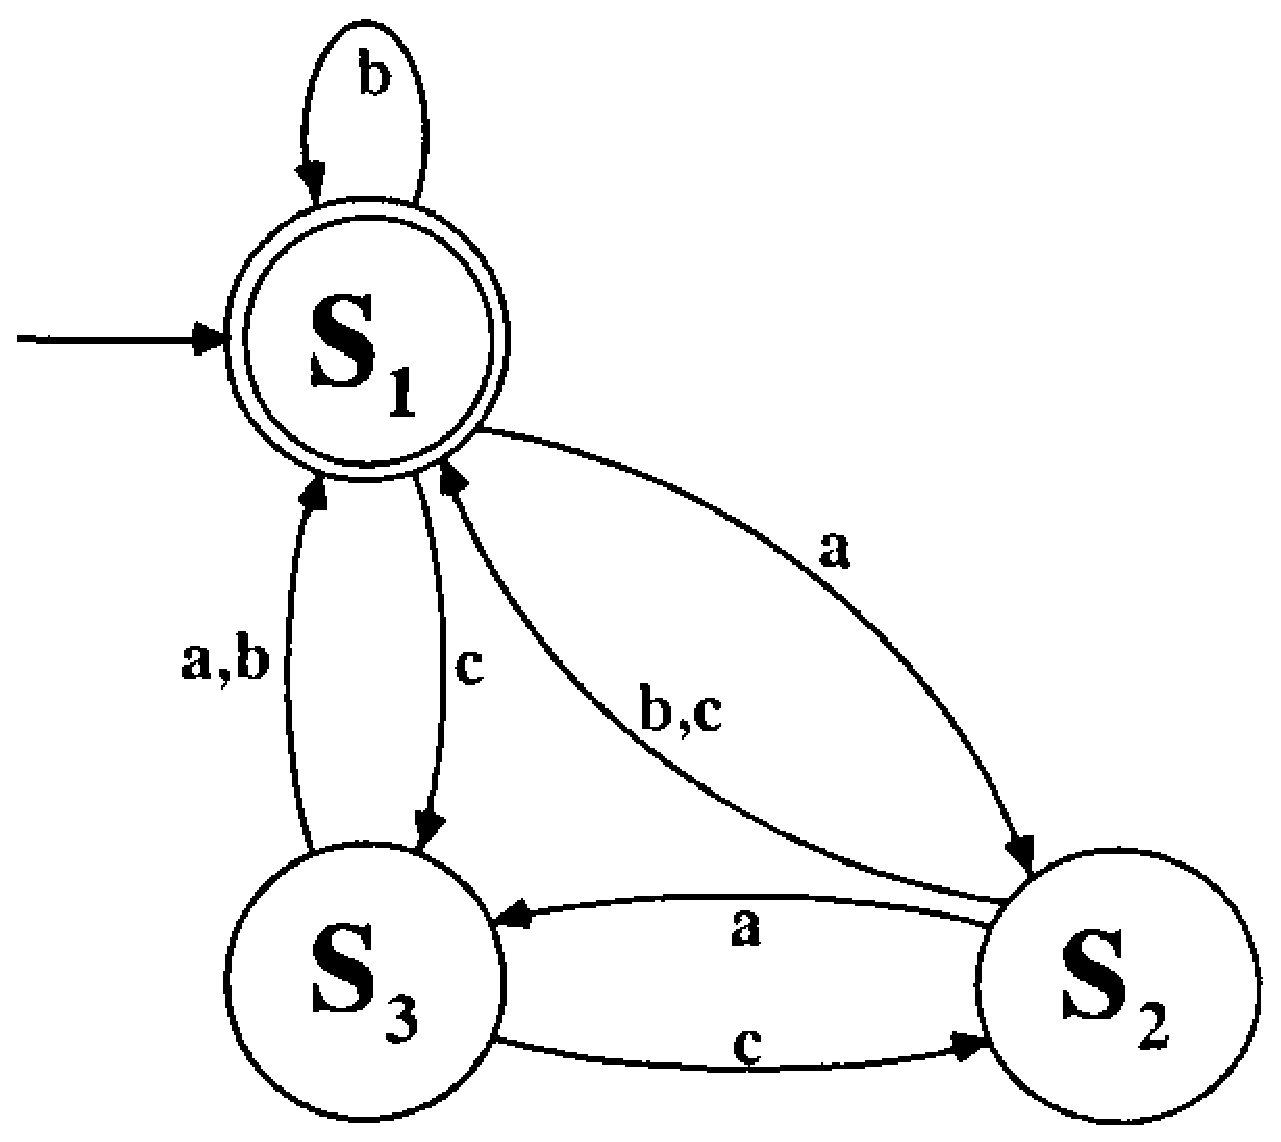
\epsfig{figure=ToFAfigures/fig6-7.eps,width=2.5in}}
\caption{The DFA discussed in Example 6.11}\label{fig-6.7}
\end{figure}

Regular expressions for machines with more than two states can be found by
repeated application of the technique described in Theorem \ref{thm-6.2}. For example,
consider the three-state DFA given in Figure \ref{fig-6.7}. The solution for this
three-state machine will be explored shortly. We begin by illustrating the
natural relationships between the terminal sets described in Theorem \ref{thm-6.3}. First
let us note that the language accepted by this machine includes:
\begin{enumerate}
\item All strings that end with $\pmb{b}$.
\item Strings that contain no $\pmb{b}$s, but for which $|x|_{\pmb{a}} -
	|x|_{\pmb{c}}$ is a multiple of 3.
\item Strings that are concatenations of type (1) and type (2) strings.
\end{enumerate}

According to Theorem \ref{thm-6.3}, the equations for this machine are
\begin{align*}
& X_1 = \epsilon \cup \pmb{b}X_1 \cup \pmb{a}X_2 \cup \pmb{c}X_3 \\
& X_2 = \emptyset \cup (\pmb{b}\cup\pmb{c})X_1 \cup \emptyset X_2 \cup \pmb{a}
	X_3 \\
& X_3 = \emptyset \cup (\pmb{a}\cup\pmb{b})X_1 \cup \pmb{c}X_2 \cup \emptyset
	X_3
\intertext{which can be simplified to}
& X_1 = \epsilon \cup \pmb{b}X_1 \cup \pmb{a}X_2 \cup \pmb{c}X_3 \\
& X_2 = (\pmb{b}\cup\pmb{c})X_1 \cup \pmb{a}X_3 \\
& X_3 = (\pmb{a}\cup\pmb{b})X_1 \cup \pmb{c}X_2
\intertext{and rewritten as}
& X_1 = \epsilon \cup \pmb{b}X_1 \cup \pmb{a}X_2 \cup \pmb{c}X_3 \\
& X_2 = \pmb{b}X_1 \cup \pmb{c}X_1 \cup \pmb{a}X_3 \\
& X_3 = \pmb{a}X_1 \cup \pmb{b}X_1 \cup \pmb{c}X_2
\end{align*}

The equation for $X_1$ admits the following interpretation; recalling that $X_1$
represents all the strings that reach a final state when starting from $s_1$, we
see that these can be broken up into four distinct classes:
\begin{enumerate}
\item Strings of length 0: $(\epsilon)$.
\item Strings that start with $\pmb{a}$ (and note that $\pmb{a}$ moves the current
	state from $s_1$ to $s_2$) and then proceed (from $s_2$) to a final
	state: $(\pmb{a}X_2)$.
\item Strings that start with $\pmb{b}$ and then proceed to a final state:
	$(\pmb{b}X_1)$.
\item Strings that start with $\pmb{c}$ and then proceed to a final state:
	$(\pmb{c}X_3)$.
\end{enumerate}
The union of these four classes should equal $X_1$, which is exactly what the
first equation states.

$X_2 = \pmb{b}X_1 \cup \pmb{c}X_1 \cup \pmb{a}X_3$ can be interpreted similarly;
$\epsilon$ does not appear in this equation because there is \emph{no} way to
reach a final state from $s_2$ if no letters are processed. If at least one
letter is processed, then that first letter is an $\pmb{a}$, $\pmb{b}$, or $\pmb{c}$.
If it is $\pmb{a}$, then we move from state $s_2$ to $s_3$, and the remainder of
the string must take us to a final state from $s_3$ (that is, the remainder must
belong to $X_3$). Strings that begin with an $\pmb{a}$ and are followed by a
string from $X_3$ can easily be described by $\pmb{a}\cdot X_3$. Similarly,
strings that start with $\pmb{b}$ or $\pmb{c}$ must move from $s_2$ to $s_1$, and
then be followed by a string from $X_1$. These strings are described by
$\pmb{b}\cdot X_1$ and $\pmb{c}\cdot X_1$. The three cases for reaching a final
state from $s_2$ that have just been described are exhaustive (and mutually
exclusive), and so their union should equal all of $X_2$. This is exactly the
relation expressed by the second equation, $X_2=\pmb{b}X_1 \cup \pmb{c}X_1 \cup
\pmb{a}X_3$. The last equation admits a similar interpretation.

None of the above observations are necessary to actually solve the system! The
preceding discussion is intended to illustrate that the natural relationships
between the terminal sets described by Theorem \ref{thm-6.3} and the correspondences we
have so laboriously developed here are succinctly predicted by the language
equations. Once the equations are written down, we can simply apply Theorem \ref{thm-6.2}
and reduce to a system with only two unknowns. We have
\begin{center}\begin{tabular}{r@{ = }l@{$\qquad$}r@{ = }l@{$\qquad$}r@{ = }l}
$E_1$ & $\epsilon$, & $E_2$ & $\emptyset$, & $E_3$ & $\emptyset$ \\
$A_{11}$ & $\pmb{b}$, & $A_{12}$ & $\pmb{a}$, & $A_{13}$ & $\pmb{c}$ \\
$A_{21}$ & $\pmb{b}\cup\pmb{c}$, & $A_{22}$ & $\emptyset$, & $A_{23}$ &
	$\pmb{a}$ \\
$A_{31}$ & $\pmb{a}\cup\pmb{b}$, & $A_{32}$ & $\pmb{c}$, & $A_{33}$ &
	$\emptyset$
\end{tabular}\end{center}
from which we can compute
\begin{center}\begin{tabular}{r@{ = }l@{$\qquad$}r@{ = }l}
$\hat{E}_1$ & $E_1 \cup A_{13}A^*_{33}E_3 = \epsilon\cup \pmb{c}\emptyset^*
	\emptyset = \epsilon,$ & $\hat{E}_2$ & $\emptyset$ \\
$\hat{A}_{11}$ & $A_{11} \cup A_{13}A^*_{33}A_{31} = \pmb{b} \cup \pmb{c}
	\emptyset^*(\pmb{a}\cup\pmb{b}) = \pmb{b}\cup\pmb{c}(\pmb{a}\cup\pmb{b}),$
	& $\hat{A}_{12}$ & $\pmb{a}\cup\pmb{c}\emptyset^*\pmb{c} = \pmb{a}\cup
	\pmb{cc}$ \\
$\hat{A}_{21}$ & $\pmb{b}\cup\pmb{c}\cup\pmb{a}\emptyset^*(\pmb{a}\cup\pmb{b}) =
	\pmb{b}\cup\pmb{c}\cup\pmb{a}(\pmb{a}\cup\pmb{b}),$ & $\hat{A}_{22}$ &
	$\emptyset\cup\pmb{a}\emptyset^*\pmb{c} = \pmb{ac}$
\end{tabular}\end{center}
which gives the following system of equations:
\begin{center}\begin{tabular}{r@{ = }l}
$X_1$ & $\epsilon\cup(\pmb{b}\cup\pmb{c}(\pmb{a}\cup\pmb{b}))X_1\cup(\pmb{a}\cup
	\pmb{cc})X_2$ \\
$X_2$ & $\emptyset\cup((\pmb{b}\cup\pmb{c})\cup\pmb{a}(\pmb{a}\cup\pmb{b}))X_1
	\cup\pmb{ac}X_2$
\end{tabular}\end{center}
These two equations can be reduced to a single equation by applying Theorem
\ref{thm-6.2} again:
\begin{center}\begin{tabular}{r@{ = }l}
$\hat{\hat{E}}_1$ & $\hat{E}_1 \cup \hat{A}_{12}(\hat{A}_{22})^*\hat{E}_2 = \epsilon
	\cup (\pmb{a}\cup\pmb{cc})\cdot(\pmb{ac})^*\cdot\emptyset = \epsilon$ \\
$\hat{\hat{A}}_{11}$ & $\hat{A}_{11}\cup\hat{A}_{12}(\hat{A}_{22})^*\hat{A}_{21} =
	\pmb{b}\cup\pmb{c}(\pmb{a}\cup\pmb{b})\cup(\pmb{a}\cup\pmb{cc})
	(\pmb{ac})^*((\pmb{b}\cup\pmb{c})\cup\pmb{a}(\pmb{a}\cup\pmb{b}))$
\end{tabular}\end{center}
which yields one equation in one unknown whose solution is
\[ X_1 = (\hat{\hat{A}}_{11})^*\hat{\hat{E}}_1 = (\pmb{b}\cup\pmb{c}(\pmb{a}\cup
	\pmb{b})\cup(\pmb{a}\cup\pmb{cc})(\pmb{ac})^*((\pmb{b}\cup\pmb{c})\cup
	\pmb{a}(\pmb{a}\cup\pmb{b})))^*\cdot\epsilon \]
Since $s_1$ was the only start state, the regular expression given by $X_1$
should describe the language accepted by the original three-state automaton.

Returning to our observations above, this expression can be reconciled with
our intuitive notion of what the solution ``should'' look like.
$\hat{\hat{A}}_{11}$ can be expanded to yield the following form:
\begin{center}\begin{tabular}{r@{ }l}
$\hat{\hat{A}}_{11} =$ & $\pmb{b}\cup\pmb{ca}\cup\pmb{cb}\cup\pmb{a}(\pmb{ac})^*
	\pmb{b}\cup\pmb{a}(\pmb{ac})^*\pmb{c}\cup\pmb{a}(\pmb{ac})^*\pmb{ab}\cup
	\pmb{a}(\pmb{ac})^*\pmb{aa}$ \\
& $\cup\,\pmb{cc}(\pmb{ac})^*\pmb{b}\cup\pmb{cc}(\pmb{ac})^*\pmb{c}\cup\pmb{cc}
	(\pmb{ac})^*\pmb{ab}\cup\pmb{cc}(\pmb{ac})^*\pmb{aa}$
\end{tabular}\end{center}
Observe that each of the 11 subexpressions consists of strings that (1) end
with $\pmb{b}$, or (2) contain no $\pmb{b}$s, but for which $|x|_{\pmb{a}} -
|x|_{\pmb{c}}$ is a multiple of 3. Hence the Kleene closure of this expression,
which represents the language accepted by this machine, does indeed agree with
our notion of what $X_1$ should describe.

Since $s_1$ is also the only final state in this example, it is interesting to
note that each of the subexpressions of $\hat{\hat{A}}_{11}$ describe strings
that, when starting at $s_1$ in the automaton, return you to $s_1$ again
\emph{for the first time} (examine the diagram and verify this).

\subsection*{Example 6.12}

Consider the automaton shown in Figure \ref{fig-6.8}. It is similar to the one in Example
6.11, but it now gives rise to four equations in four unknowns. As these
equations are solved, the final $\hat{\hat{\hat{A}}}_{11}$ coefficient for $X_1$
will again describe strings that, when starting at $s_1$ in the automaton,
return you to $s_1$ again for the first time; it will agree with
${\hat{\hat{A}}}_{11}$ in Example 6.11. The final constant term associated
with $X_1$ (that is, $\hat{\hat{\hat{E}}}_1$), will represent all those strings
that deposit you in a final state from $s_1$ without ever returning to $s_1$. In
this automaton, this will be given by $\hat{\hat{\hat{E}}}_1 = \pmb{de}^*$\!\!. \ 
$\hat{\hat{\hat{A}}}^*_{11}\hat{\hat{\hat{E}}}_1$ therefore represents strings
that go from $s_1$ back to $s_1$ any number of times, followed by a string that
leaves $s_1$ (for the last time) for a final state.

% Figure 6.8
\begin{figure}
\centerline{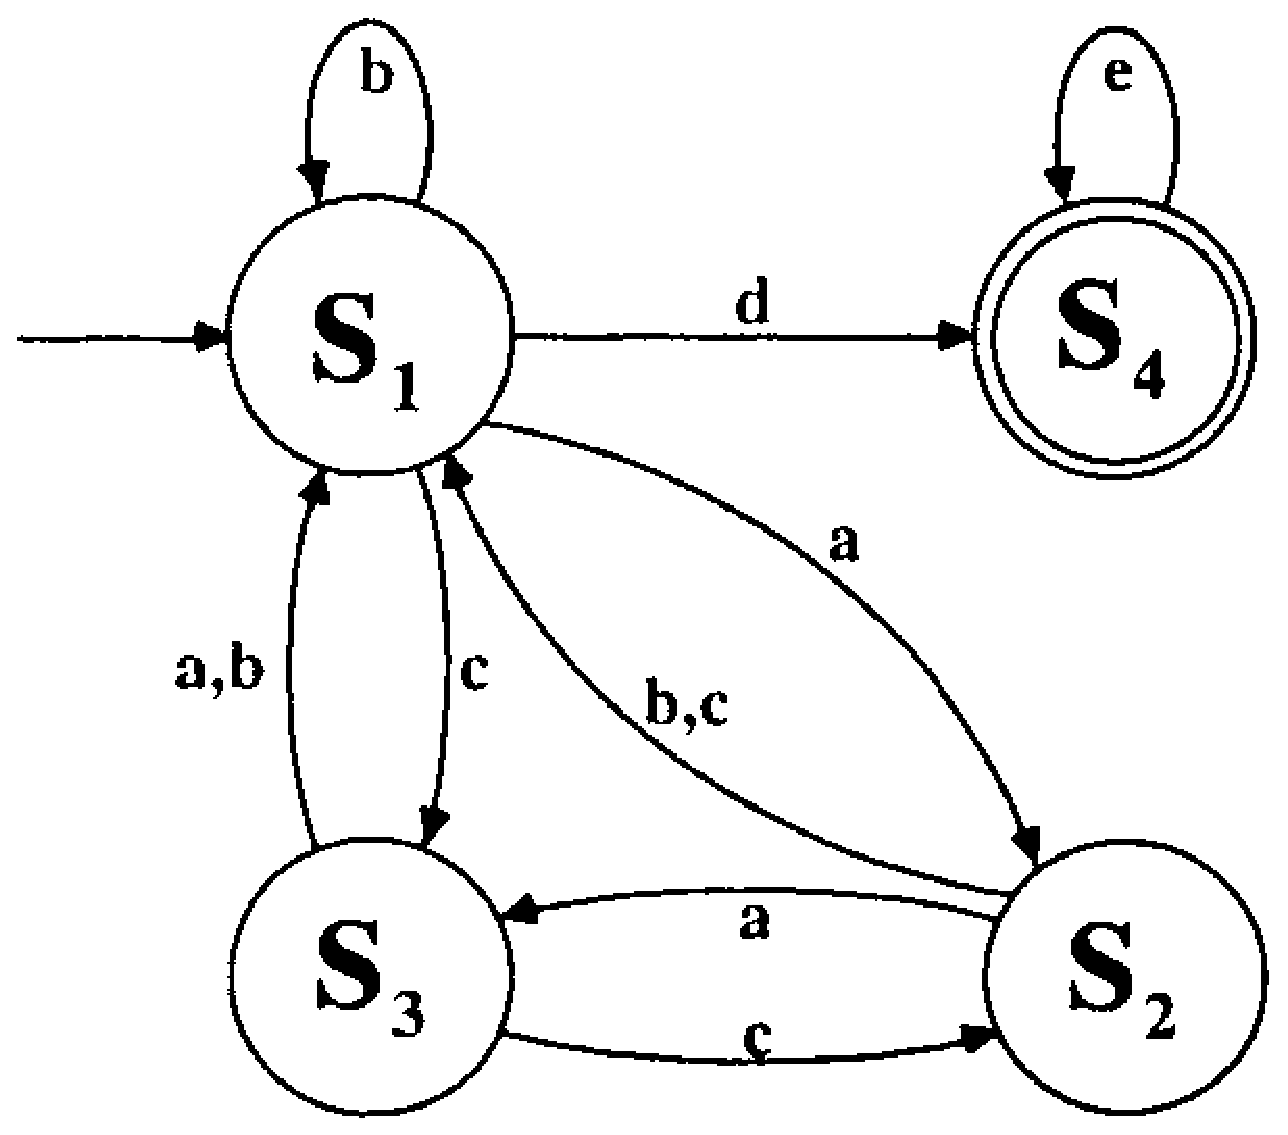
\epsfig{figure=ToFAfigures/fig6-8.eps,width=2.5in}}
\caption{The DFA discussed in Example 6.12}\label{fig-6.8}
\end{figure}

In general, the final coefficient and constant terms can always be interpreted
in this manner. In Example 6.11, the only way to reach a final state from $s_1$
and avoid having to return again to $s_1$ was to not leave in the first place;
this was reflected by the fact that $\hat{\hat{E}}_1 = \epsilon$.

\subsection*{Example 6.13}

% Figure 6.9
\begin{figure}
\centerline{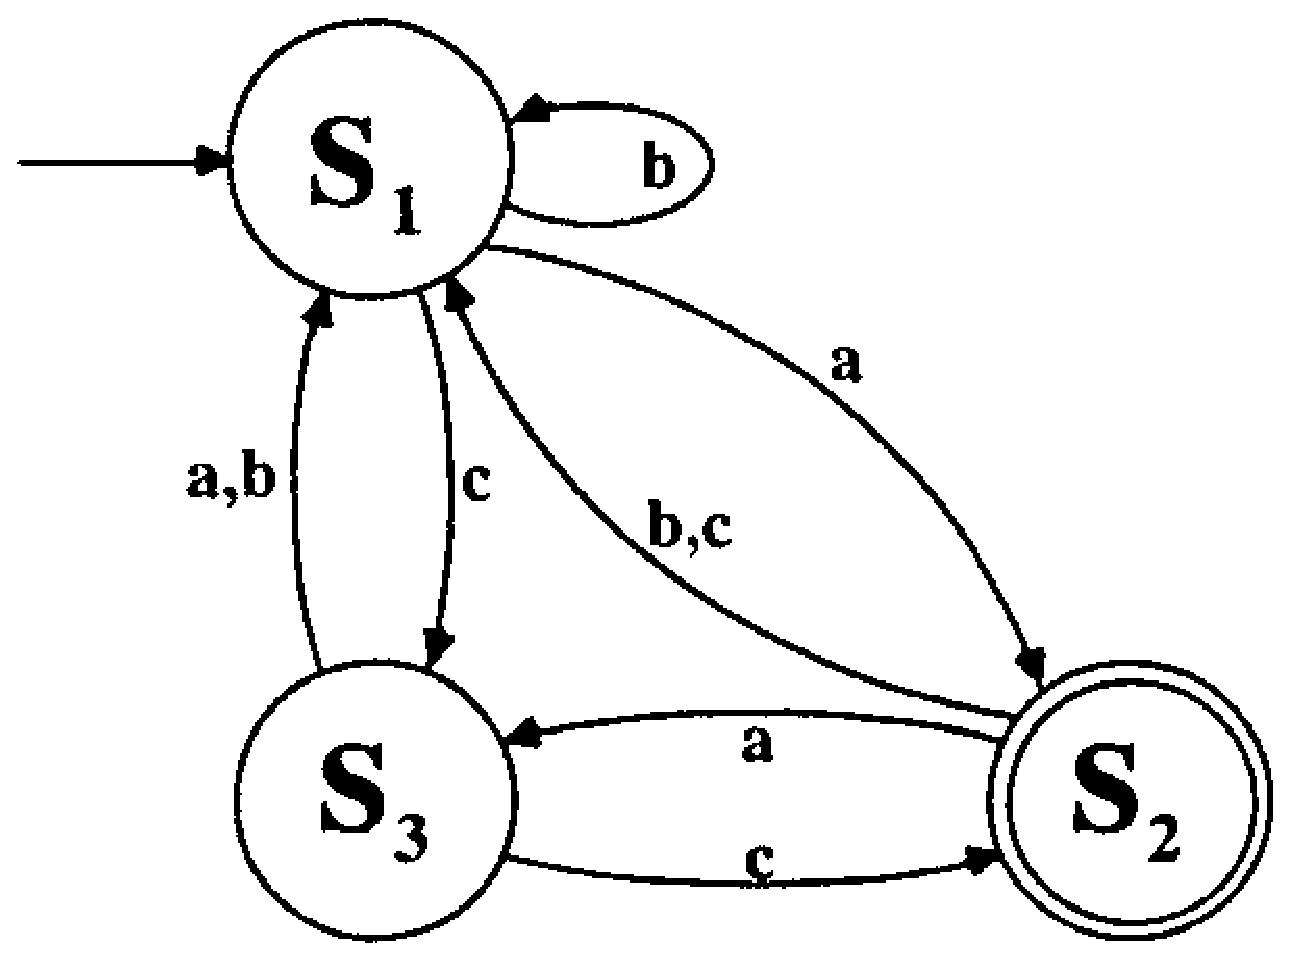
\epsfig{figure=ToFAfigures/fig6-9.eps,width=2.5in}}
\caption{The DFA discussed in Example 6.13}\label{fig-6.9}
\end{figure}

Consider the automaton illustrated in Figure \ref{fig-6.9}, which is identical to the
DFA in Example 6.11 except for the placement of the final state. Even though the
initial system of three equations is now different, we can expect
$\hat{\hat{A}}_{11}$ to compute to the same expression as before. Since
$\hat{\hat{E}}_1$ is supposed to represent all those strings that deposit you in
a final state from $s_1$ without ever returning to $s_1$, one should be able to
predict that the new final constant term will look like $\hat{\hat{E}}_1 =
\pmb{a}(\pmb{ac})^*\cup\pmb{c}(\pmb{ca})^*\pmb{c}$. An expression for the
language recognized by this automaton would then be given by

\begin{center}\begin{tabular}{r@{ = }l}
$X_1$ & $(\hat{\hat{A}}_{11})^*\hat{\hat{E}}_1$ \\
& $(\pmb{b}\cup\pmb{c}(\pmb{a}\cup\pmb{b})\cup(\pmb{a}\cup\pmb{cc})(\pmb{ac})^*
	((\pmb{b}\cup\pmb{c})\cup\pmb{a}(\pmb{a}\cup\pmb{b})))^*\cdot(\pmb{a}
	(\pmb{ac})^*\cup\pmb{c}(\pmb{ca})^*\pmb{c})$
\end{tabular}\end{center}

It may often be convenient to eliminate a variable other than the one that is
numerically last. This can be accomplished by appropriately renumbering the
unknowns and applying Theorem \ref{thm-6.2} to the new set of equations. For convenience,
we state an analog of Theorem \ref{thm-6.2} that allows the elimination of the $m^\text{th}$
unknown from a set of $n$ equations in $n$ unknowns. The following lemma agrees
with Theorem \ref{thm-6.2} if $m = n$.

% Lemma 6.3
\begin{lmm}\label{lmm-6.3}
Let $n$ and $m$ be positive integers and let $m \leq n$. Consider the system of
$n \geq 2$ equations in the unknowns $X_1,X_2,\ldots,X_n$, given by
\[ X_k = E_k \cup A_{k1}X_1 \cup A_{k2}X_2 \cup\cdots\cup A_{kn}X_n,\qquad
	\text{for }k = 1,2, \ldots , n \]
in which $(\forall i,j)(\lambda \notin A_{ij})$

The unknown $X_m$ can be eliminated from this system to form the following $n-1$
equations in the unknowns $X_1,X_2,\ldots,X_{m-1},X_{m+1},\ldots,X_n$.
\begin{center}\begin{tabular}{r@{ }l}
$X_k =$ & $\hat{E}_k \cup \hat{A}_{k1}X_1 \cup \hat{A}_{k2}X_2 \cup\ldots\cup
	\hat{A}_{k(m-1)}X_{m-1}\cup\hat{A}_{k(m+1)}X_{m+1}\cup\ldots\cup
	\hat{A}_{kn}X_n$, \\
& for $k = 1, 2,\ldots,m-1,m+1, \ldots ,n$
\end{tabular}\end{center}
where
\[ \hat{E}_i = E_i \cup (A_{im}\cdot A^*_{mm}\cdot E_m),\qquad\text{for all }
	i = 1,2, \ldots ,m-1,m+1, \ldots ,n \]
and
\[ \hat{A}_{ij} = A_{ij} \cup (A_{im}\cdot A^*_{mm}\cdot A_{mj}),\qquad
	\text{for all }i,j = 1,2, \ldots ,m-1,m+1, \ldots ,n \]
Furthermore, once the solution to the above $n-1$ equations is known, that
solution can be used to find the remaining unknown:
\begin{center}\begin{tabular}{r@{ }l}
$X_m =$ & $A^*_{mm} \cdot (E_m \cup A_{m1}X_1 \cup A_{m2}X_2 \cup\ldots\cup
	A_{m(m-1)}X_{m-1}$ \\
& $\cup\, A_{m(m+1)}X_{m+1}\cup\ldots\cup A_{mn}X_n)$
\end{tabular}\end{center}

\emph{Proof.} The proof follows from a renumbering of the equations given in
Theorem \ref{thm-6.2}.
\end{lmm}

% Figure 6.10
\begin{figure}
\centerline{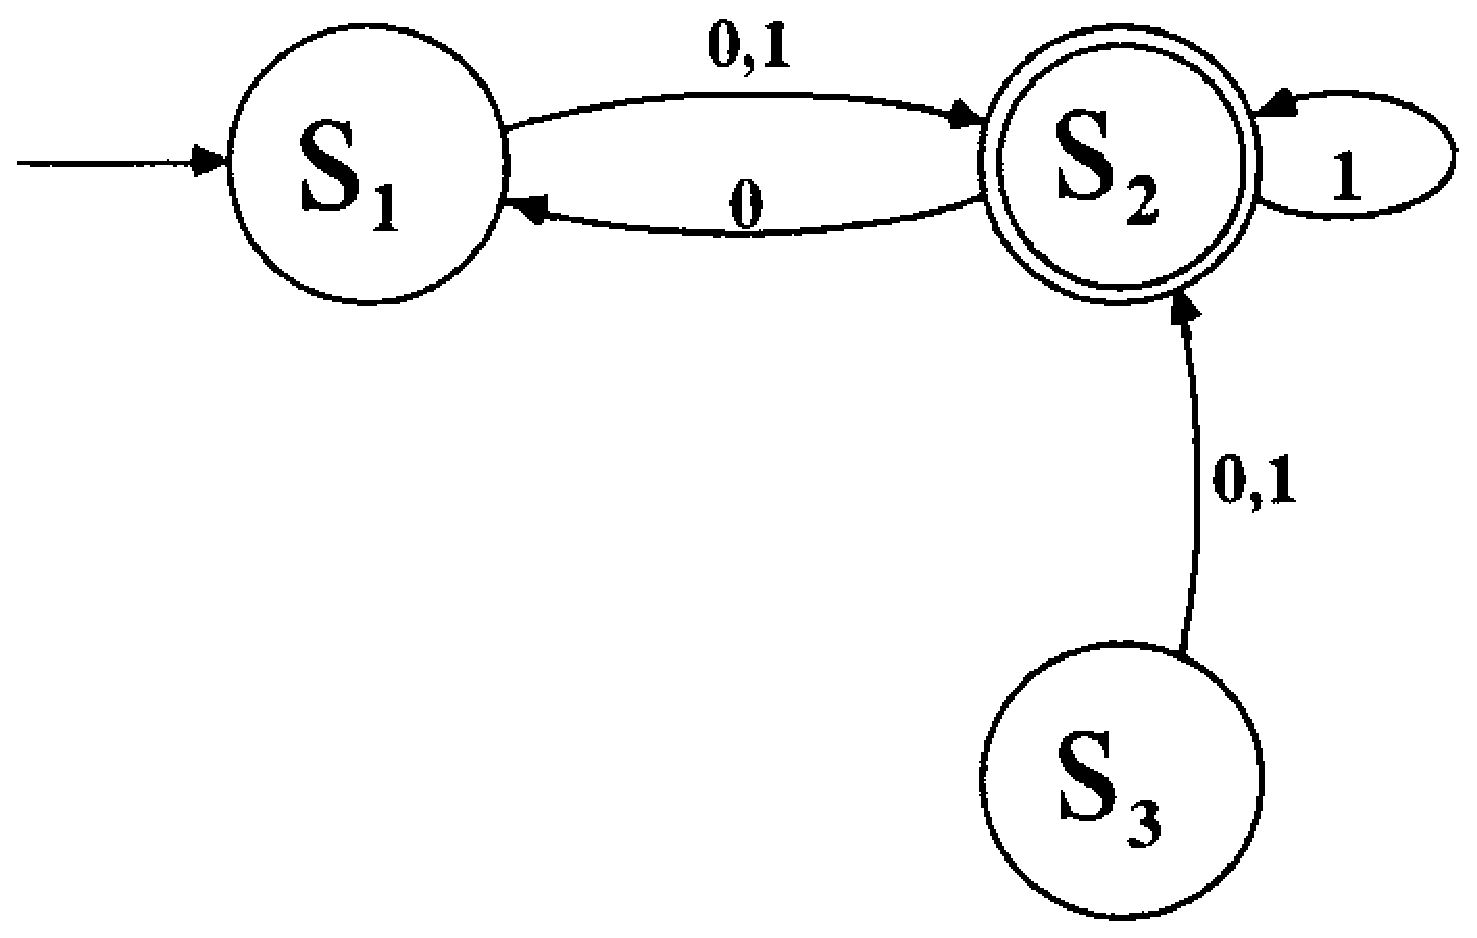
\epsfig{figure=ToFAfigures/fig6-10.eps,width=2.5in}}
\caption{The DFA discussed in Exercise 6.19}\label{fig-6.10}
\end{figure}

A significant reduction in the size of the expressions representing the
solutions can often be achieved by carefully choosing the order in which to
eliminate the unknowns. This situation can easily arise when solving language
equations that correspond to finite automata. For example, consider the DFA
illustrated in Figure \ref{fig-6.10}. The equations for this machine are given by
\begin{center}\begin{tabular}{r@{ = }l}
$X_1$ & $\emptyset\cup\emptyset X_1 \cup (\pmb{0}\cup\pmb{1})X_2\cup\emptyset
	X_3$ \\
$X_2$ & $\epsilon \cup \pmb{0} X_1 \cup \pmb{1}X_2 \cup \emptyset X_3$ \\
$X_3$ & $\emptyset\cup\emptyset X_1 \cup (\pmb{0}\cup\pmb{1})X_2\cup\emptyset
	X_3$
\end{tabular}\end{center}
Using Theorem \ref{thm-6.2} to methodically solve for $X_1$, $X_2$, and $X_3$ involves
eliminating $X_3$ and then eliminating $X_2$. Theorem \ref{thm-6.1} can then be used to
solve for $X_1$, and then the back-substitution rules can be employed to find
$X_2$ and $X_3$. The regular expressions found in this manner are quite complex.
A striking simplification can be made by eliminating $X_3$ and then eliminating
$X_1$ (instead of $X_2$) . The solution for $X_2$ is quite concise, which leads
to simple expressions for $X_1$ and $X_3$ during the back-substitution phase (see
Exercise 6.19).

Let $A=\langle\Sigma,\{s_1,s_2,\ldots,s_n\},s_1,\delta,F\rangle$ be a
deterministic finite automaton. We have seen that the relationships between the
terminal sets $T(A,s_i)$ described in Chapter \ref{ch-3} give rise to a system of
equations. Similarly, the initial sets $I(A,s_i)$ defined in Chapter \ref{ch-2} are also
interrelated. Recall that, for a state $s_i$, $I(A,s_i)$ is comprised of strings
that, when starting in the start state, lead to the state $s_i$. That is,
$I(A,s_i)=\{x\ \ |\ \DBAR(s_1,x) = s_i\}$. The equations we have discussed to this
point have been \emph{\Index{right linear}}; that is, the unknowns $X_i$ appear
to the right of their coefficients. The initial sets for an automaton are also
related by a system of equations, but these equations are \emph{\Index{left
linear}}; the unknowns $Y_i$ appear to the left of their coefficients. The
solution for sets of left-linear equations parallels that of right-linear
systems.

% Theorem 6.4
\begin{thm}\label{thm-6.4}
Let $n$ and $m$ be positive integers and let $m \leq n$. Consider the system of
$n \geq 2$ equations in the unknowns $Y_1,Y_2,\ldots,Y_n$ given by
\[ Y_k = I_k\cup Y_1B_{k1} \cup Y_2B_{k2} \cup\cdots\cup Y_nB_{kn},\qquad
	\text{for }k = 1,2,\ldots,n \]
in which $(\forall i,j)(\lambda \notin B_{ij})$.
\begin{enumerate}[a.]
\item The unknown $Y_m$ can be eliminated from this system to form the following
$n-1$ equations in the unknowns $Y_1,Y_2, \ldots , Y_{m-1},Y_{m+1},\ldots,Y_n$.
\[ Y_k = \hat{I}_k \cup Y_1\hat{B}_{k1} \cup Y_2\hat{B}_{k2} \cup\cdots\cup
	Y_{m-1}\hat{B}_{k(m-1)}\cup Y_{m+1}\hat{B}_{k(m+1)} \cup\cdots\cup
	Y_n\hat{B}_{kn}, \]
for $k = 1,2, \ldots ,m-1,m+1,\ldots, n$ \\
where
\[ \hat{I}_i=  I_i \cup(I_m \cdot B^*_{mm} \cdot B_{im}),\qquad\text{for all }
	i = 1,2,\ldots,m-1,m+1,\ldots,n \]
and
\[ \hat{B}_{ij} = B_{ij} \cup (B_{mj}\cdot B^*_{mm} \cdot B_{im}),\qquad
	\text{for all }i,j = 1,2,\ldots,m-1,m+1,\ldots,n \]

\item Once the solution to the above $n - 1$ equations is known, that solution
can be used to find the remaining unknown:
\begin{center}\begin{tabular}{r@{ }l}
$Y_m =$ & $(I_m \cup Y_1B_{m1} \cup Y_2B_{m2} \cup\cdots\cup Y_{m-1}B_{m(m-1)}$ \\
& $\cup\, Y_{m+1}B_{m(m+1)} \cup\cdots\cup Y_nB_{mn})\cdot B^*_{mm}$
\end{tabular}\end{center}

\item A single equation $Y_1=I_1 \cup Y_1B_{11}$ has the unique solution
$Y_1 = I_1B^*_{11}$.
\end{enumerate}

\emph{Proof.} The proof is essentially a mirror image of the proofs given in
Theorems \ref{thm-6.1} and \ref{thm-6.2}.
\end{thm}

% Lemma 6.4
\begin{lmm}\label{lmm-6.4}
Let $A=\langle\Sigma,\{s_1,s_2,\ldots,s_n\},S_0,\delta,F\rangle$ be an NDFA. For
each $i=1,2,\ldots,n$, let the initial set $I(A,s_i)=\{x\ |\ \DBAR(s_1,x) = s_i\}$
be denoted by $Y_i$. The unknowns $Y_1,Y_2,\ldots,Y_n$ satisfy a system of $n$
left-linear equations of the form
\[ Y_k = I_k \cup Y_1B_{k1} \cup Y_2B_{k2} \cup\cdots\cup Y_nB_{kn},\qquad
	\text{for }k = 1,2,\ldots,n \]
where the coefficients are given by
\begin{align*}
I_i = & \left\{ \begin{tabular}{ll}
			$\emptyset$ & if $s_i \notin S_0$ \\
			& \\
			$\epsilon$ & if $s_i \in S_0$
		 \end{tabular}\right. &
		 \text{for }i = 1,2,\ldots,n \\
\intertext{and}
B_{ij} = & \bigcup\limits_{\pmb{a}\,\in\,\Sigma\,\wedge\,s_i\,\in\,\delta(s_j,
	\pmb{a})} \pmb{a} & \text{for }i,j=1,2, \ldots ,n
\end{align*}

\emph{Proof.} See the exercises.
\end{lmm}

In contrast to Theorem \ref{thm-6.3}, where $A_{ij}$ represented the set of all letters
that causes a transition from state $s_i$ to state $s_j$, $B_{ij}$ represents
the set of all letters that causes a transition from state $s_j$ to state $s_i$.
That is, $B_{ij} = A_{ji}$. In the definition in Theorem \ref{thm-6.3}, $E_i$ represented
the set of all strings of length zero that can reach final states from $s_i$.
Compare this with the definition of $I_i$ above, which represents the set of all
strings of length zero that can reach $s_i$ from a start state.

\section{FAD Languages As Regular Sets; Closure Properties}\label{sec-6.4}

The technique outlined by Theorems \ref{thm-6.1}, \ref{thm-6.2}, and \ref{thm-6.3}
provide the second half of the correspondence between regular sets and FAD
languages. As a consequence, regular expressions and automata characterize
exactly the same class of languages.

% Corollary 6.2
\begin{cor}\label{cor-6.2}
Let $\Sigma$ be an alphabet. Then $\DSIG \subseteq \RSIG$.

\emph{Proof.} The proof follows immediately from Theorem \ref{thm-6.3}.
\end{cor}

% Theorem 6.5
\begin{thm}\label{thm-6.5}\index{equivalent!regular expressions}
{\bf \Index{Kleene's Theorem}}. Let $\Sigma$ be an alphabet. Then $\RSIG = \DSIG$.

\emph{Proof.} The proof follows immediately from Corollaries 6.1 and 6.2.
\end{thm}

Thus the terms \emph{FAD language} and \emph{regular set} can be used
interchangeably, since languages accepted by finite automata can be described by
regular expressions, and vice versa. Such languages are often referred to as
\emph{\Index{regular language}s}. The correspondence will allow, for example,
the pumping lemma to be invoked to justify that certain languages cannot be
represented by any regular expression.

\RSIG\ is therefore closed under every operator for which \DSIG\ is closed. We
have now seen two representations for FAD languages, and a third will be
presented in Chapter \ref{ch-8}. Since there are effective algorithms for switching from
one representation to another, we may use whichever vehicle is most convenient
to describe a language or prove properties about regular languages. For example,
we may use whichever concept best lends itself to the proof of closure
properties. The justification that \RSIG\ is closed under union follows
immediately from Definition \ref{dfn-6.1}; much more effort was required in Chapter \ref{ch-5} to
prove that the union of two languages represented by DFAs could be represented
by another DFA. On the other hand, attempting to justify closure under
complementation by using regular expressions is an exercise in frustration. We
will now see that closure under \emph{substitution} is conveniently
proved via regular expressions.

A substitution is similar to a language homomorphism (Definition \ref{dfn-5.8}), in
which letters were replaced by single words. Substitutions will denote the
methodical replacement of the individual letters within a regular expression
with \emph{sets} of words. The only restriction on these sets is that they must
also be regular expressions, though not necessarily over the same alphabet.

% Definition 6.5
\begin{dfn}\label{dfn-6.5}\index{substitution!regular set}
Let $\Sigma=\{\pmb{a}_1,\pmb{a}_2,\ldots,\pmb{a}_m\}$ be an alphabet and let
$\Gamma$ be a second alphabet. Given regular expressions $R_1,R_2,\ldots,R_m$
over $\Gamma$, define a \emph{\Index{regular set substitution}} $s$$:\Sigma
\rightarrow \wp(\Gamma^*)$ by $s(\pmb{a}_i) = R_i$ for each $i=1,2,\ldots,m$,
which can be extended to $\overline{s}:\ \Sigma^* \rightarrow \wp(\Gamma^*)$ by
\[ \overline{s}(\lambda) = \epsilon \]
and
\[ (\forall\pmb{a}\in\Sigma)(\forall x \in\Sigma^*)(\overline{s}(\pmb{a}\cdot x)
	= s(\pmb{a})\cdot \overline{s}(x)) \]
$\overline{s}$ can be further extended to operate on a language $L \subseteq
\Sigma^*$ by defining
\[ \overline{s}(L) = \bigcup\limits_{z\,\in\, L} \overline{s}(z) \]
In this last context, $\overline{s}:\ \wp(\Sigma^*) \rightarrow \wp(\Gamma^*)$.
\end{dfn}

\subsection*{Example 6.14}

Let $\Sigma=\{\pmb{0}\}$ and $\Gamma=\{\pmb{a},\pmb{b}\}$. Define $s(\pmb{0}) =
(\pmb{a}\cup\pmb{b})\cdot(\pmb{a}\cup\pmb{b})$. From the recursive definition,
$\overline{s}(\pmb{00}) = (\pmb{a}\cup\pmb{b})\cdot(\pmb{a}\cup\pmb{b})\cdot
(\pmb{a}\cup\pmb{b})\cdot(\pmb{a}\cup\pmb{b})$. Furthermore, the language
$\overline{s}(\pmb{0}^*)$ represents all even-length strings over $\{\pmb{a},
\pmb{b}\}$.

The definition of $\overline{s}(L)$ for a language $L$ allows the domain of the
substitution to be extended all the way to $\overline{s}$$: \wp(\Sigma^*) \rightarrow \wp
(\Gamma^*)$. It can be proven that the image of \RSIG\ under $\overline{s}$ is
contained in $\mathfrak{R}_{\Gamma}$ (see the exercises); however, the image of
\NSIG\ under $\overline{s}$ is not completely contained in $\mathfrak{N}_{\Gamma}$

In Example 6.14, the language $\pmb{0}^*$ was regular and so was its image under
$\overline{s}$. %Neither of the sets described in the second example were regular.
It is possible to start with a nonregular set and define a substitution that
produces a regular set (see Lemma \ref{lmm-6.5}), but it is impossible for the image of a
regular set to avoid being regular, as shown by the next theorem.

% Theorem 6.6
\begin{thm}\label{thm-6.6}\index{closure!under substitution}
Let $\Sigma$ be an alphabet, and let $s:\ \Sigma \rightarrow \wp(\Sigma^*)$ be a
substitution. Then \RSIG\ is closed under $\overline{s}$.

\emph{Proof.} Choose an arbitrary regular expression $R$ over $\Sigma$. We must
show that $\overline{s}(R)$ represents a regular set. $R$ is an expression made
up of the letters in $\Sigma$ and the characters $(,),\cup$, and $^*$. Form the
new expression $R'$ by replacing each letter $\pmb{a}$ by $s(\pmb{a})$. $R'$ is
then clearly another regular expression over $\Sigma$. In fact, it can be shown
that $R'$ represents exactly the words in $\overline{s}(R)$; this is formally
accomplished by inducting on the number of operators in the expression $R$. To
prove this, one must argue that this substitution correspondence is preserved by
each of the six rules defining regular expressions. The basis step of the
induction involves all regular expressions with zero operators, that is, those
defined by the first three rules for generating a regular expression.
\begin{enumerate}[i.]
\item The substitution corresponding to any single letter $\pmb{a}_i$ is a
regular expression corresponding to $\overline{s}(\pmb{a}_i)$, since, by
definition of $\overline{s}$, $\overline{s}(\pmb{a}_i) = s(\pmb{a}_i)$.
\item The substitution corresponding to $\emptyset$ is a regular expression
corresponding to $\overline{s}(\emptyset)$, since, by definition of
$\overline{s}$, $\overline{s}(\emptyset) = \emptyset$.
\item The substitution corresponding to $\epsilon$ is a regular expression
corresponding to $\overline{s}(\lambda)$, since, by definition of $\overline{s}$,
$\overline{s}(\lambda) = \epsilon$.
\end{enumerate}
The inductive step requires an argument that the correspondence is preserved
whenever another of the three operators is introduced to form a more complex
expression. These assertions involve the final three rules for generating
regular expressions.
\begin{enumerate}[i.]
\setcounter{enumi}{3}
\item If $R_1$ and $R_2$ are regular expressions, then the substitution
corresponding to $(R_1\cdot R_2)$ is a regular expression representing the
concatenation of the two corresponding substitutions. That is, $\overline{s}(R_1
\cdot R_2) = \overline{s}(R_1)\cdot\overline{s}(R_2)$.
\item If $R_1$ and $R_2$ are regular expressions, then the substitution
corresponding to $(R_1 \cup R_2)$ is a regular expression representing
$\overline{s}(R_1)\cup\overline{s}(R_2)$.
\item If $R_1$ is a regular expression, then the substitution corresponding to
$(R_1)^*$ is a regular expression representing $(\overline{s}(R_1))^*$.
\end{enumerate}
Each of these three assertions follows immediately from the definition of
substitution and is left as an exercise. The inductive step guarantees that
the substitution correspondence is preserved in any regular expression $R$,
regardless of the number of operators in $R$. Consequently, $R'$ is indeed a
regular expression denoting $\overline{s}(R)$, and \RSIG\ is therefore closed
under $\overline{s}$.
\end{thm}

The analogous result does \emph{not} always hold for the nonregular sets.
% Lemma 6.5
\begin{lmm}\label{lmm-6.5}
Let $\Sigma$ be an alphabet.
\begin{enumerate}[a.]
\item There are examples of regular set substitutions $s:\ \Sigma \rightarrow
	\wp(\Sigma^*)$ for which \NSIG\ is not closed under $\overline{s}$.
\item There are examples of regular set substitutions $t:\ \Sigma \rightarrow
	\wp(\Sigma^*)$ for which \NSIG\ is closed under $\overline{t}$.
\end{enumerate}

\emph{Proof.} (a) \NSIG\ is \emph{not} closed under some substitutions. Let
$\Sigma=\{\pmb{a},\pmb{b}\}$ and define $s(\pmb{a})=(\pmb{a}\cup\pmb{b})$ and
$s(\pmb{b})=(\pmb{a}\cup\pmb{b})$. The image of the nonregular set
\[ L = \{x\ | \  |x|_{\pmb{a}} = |x|_{\pmb{b}}\} \]
is the set of even-length words, which \emph{is} regular. Thus $L \in \NSIG$ but
$\overline{s}(L) \notin \NSIG$.

(b) \NSIG\ \emph{is} closed under some substitutions. Some substitutions do
preserve nonregularity (such as the identity substitution $i$, since for any
language $L$, $\overline{i}(L) = L$). In this case, $(\forall L)(L \in \NSIG
\Rightarrow \overline{i}(L)\in \NSIG)$ and therefore \NSIG\ is closed under
$\overline{i}$.
\end{lmm}
Note that a substitution in which each $R_i$ is a single string then conforms to
Definition \ref{dfn-5.8} and represents a language homomorphism.

% Corollary 6.3
\begin{cor}\label{cor-6.3}\index{closure!under language homomorphism}
Let $\Sigma$ be an alphabet, and let $\psi:\ \Sigma \rightarrow \Sigma^*$ be a
language homomorphism. Then \RSIG\ is closed under \PBAR.

\emph{Proof.} The proof follows immediately from Theorem \ref{thm-6.6}, since a language
homomorphism is a special type of substitution.
\end{cor}

As in Chapter \ref{ch-5}, this result can also be proved by successfully modifying an
appropriate DFA, showing that $\DSIG ( = \RSIG)$ is closed under language
homomorphism. It is likewise possible to use machine constructs to show that
\DSIG\ is closed under substitution, but this becomes much more complex than the
argument given for Theorem \ref{thm-6.6}. A third characterization of regular languages
will be presented in Chapter \ref{ch-8}, affording a choice of three distinct avenues for
proving closure properties of \RSIG.

\section*{Exercises}
\begin{enumerate}[{6.}1.]
\item Let $\Sigma=\{\pmb{a},\pmb{b}\}$. Give (if possible) a regular expression
that describes the set of all even-length words in $\Sigma^*$.

\item Let $\Sigma=\{\pmb{a},\pmb{b}\}$. Give (if possible) a regular expression
that describes the set of all words $x$ in $\Sigma^*$ for which $|x| \geq 2$.

\item Let $\Sigma=\{\pmb{a},\pmb{b}\}$. Give (if possible) a regular expression
that describes the set of all words $x$ in $\Sigma^*$ for which $|x|_{\pmb{a}} =
|x|_{\pmb{b}}$.

\item Let $\Sigma=\{\pmb{a},\pmb{b},\pmb{c}\}$. Give a regular expression that
describes the set of all odd-length words in $\Sigma^*$ that do not end in $\pmb{b}$.

\item Let $\Sigma=\{\pmb{a},\pmb{b},\pmb{c}\}$. Give a regular expression that
describes the set of all words in $\Sigma^*$ that do \emph{not} contain
two consecutive $\pmb{c}$s. 

\item Let $\Sigma=\{\pmb{a},\pmb{b},\pmb{c}\}$. Give a regular expression that
describes the set of all words in $\Sigma^*$ that \emph{do} contain
two consecutive $\pmb{c}$s.

\item Let $\Sigma=\{\pmb{a},\pmb{b},\pmb{c}\}$. Give a regular expression that
describes the set of all words in $\Sigma^*$ that do \emph{not} contain
\emph{any} $\pmb{c}$s.

\item Let $\Sigma=\{\pmb{0},\pmb{1}\}$. Give, if possible, regular expressions
that will describe each of the following languages. Try to write these directly
from the descriptions (that is, avoid relying on the nature of the corresponding
automata).
\begin{enumerate}
\item $L_1 = \{x\ |\ \ \ |x| \bmod{3} = 2\}$
\item $L_2 = \Sigma^* - \{w\ |\ \exists n \geq 1 \ni w = a_1\ldots a_n \wedge a_n
	= \pmb{1}\}$
\item $L_3 = \{y\ |\ \ \ |y|_{\pmb{0}} > |y|_{\pmb{1}}\}$
\end{enumerate}

\item Let $\Sigma=\{\pmb{a},\pmb{b},\pmb{c}\}$. Give, if possible, regular
expressions that will describe each of the following languages. Try to write
these directly from the descriptions (that is, avoid relying on the nature of
the corresponding automata).
\begin{enumerate}
\item $L_1 = \{x\ |\ \ \ (|x|_{\pmb{a}}$ is odd$)\wedge(|x|_{\pmb{b}}$ is even$)\}$
\item $L_2 = \{y\ |\ \ \ (|y|_{\pmb{c}}$ is even$)\vee(|y|_{\pmb{b}}$ is odd$)\}$
\item $L_3 = \{z\ |\ \ \ (|z|_{\pmb{a}}$ is even$)\}$
\item $L_4 = \{z\ |\ \ \ |z|_{\pmb{c}}$ is a prime number$\}$
\item $L_5 = \{x\ |\ \pmb{abc}$ is a substring of $x\}$
\item $L_6 = \{x\ |\ \pmb{acaba}$ is a substring of $x\}$
\item $L_7 = \{x \in \{\pmb{a},\pmb{b},\pmb{c}\}^*|\ \ \ |x|_{\pmb{a}} \equiv 0
	\bmod{3}\}$
\end{enumerate}

\item Let $\Sigma=\{\pmb{a},\pmb{b},\pmb{d}\}$. Give a regular expression that
will describe
\[ \Psi = \{x \in \Sigma^*\ |\ (x\text{ begins with }\pmb{d})\vee(x\text{ contains
	two consecutive $\pmb{b}$s})\}. \]

\item Let $\Sigma=\{\pmb{a},\pmb{b},\pmb{c}\}$. Give a regular expression that
will describe
\[ \Phi = \{x \in \Sigma^*\ |\ \text{every $\pmb{b}$ in $x$ is immediately followed
	by }\pmb{c}\}. \]

\item Let $\Sigma=\{\pmb{0},\pmb{1},\pmb{2},\pmb{3},\pmb{4},\pmb{5},\pmb{6},
\pmb{7},\pmb{8},\pmb{9}\}$. Give a regular expression that will describe
\begin{center}\begin{tabular}{r@{ = }l}
$\Gamma$ & $\{x \in \Sigma^*|\ $the number represented by $x$ is evenly
	divisible by $3\}$ \\
& $\{\lambda,\pmb{0},\pmb{00},\pmb{000},\ldots,\pmb{3},\pmb{03},\pmb{003},
	\ldots,\pmb{6},\pmb{9},\pmb{12},\pmb{15},\ldots\}$.
\end{tabular}\end{center}

\item Let $\Sigma = \{\pmb{0},\pmb{1},\pmb{2},\pmb{3},\pmb{4},\pmb{5},\pmb{6},
\pmb{7},\pmb{8},\pmb{9}\}$. Give a regular expression that will describe
\[ K = \{x \in \Sigma^*|\ \text{the number represented by $x$ is evenly divisible
	by }5\}. \]

\item Use the \emph{exact} constructs given in the theorems of Chapter \ref{ch-5} to build a
NDFA that accepts $\pmb{b}\cup\pmb{a}^*\pmb{c}$ (refer to Examples 6.4,
6.5, and 6.6). Do \emph{not} simplify your answer.

\item Give examples of sets that demonstrate the following inequalities listed
in Lemma \ref{lmm-6.1}:
\begin{enumerate}
\item $R_1 \cup \epsilon \neq R_1$
\item $R_1 \cdot R_2 \not= R_2 \cdot R_1$
\item $R_1 \cdot R_1 \not= R_1$
\item $R_1 \cup (R_2 \cdot R_3) \not= (R_1 \cup R_2)\cdot(R_1 \cup R_3)$
\item $(R_1 \cdot R_2)^* \not= (R^*_1 \cdot R^*_2)^*$
\item $(R_1 \cdot R_2)^* \not= (R^*_1 \cup R^*_2)^*$
\end{enumerate}
Find other examples of sets that show the following expressions may be equal
under some conditions:
\begin{enumerate}
\setcounter{enumii}{6}
\item $R_1 \cup \epsilon = R_1$
\item $R_1 \cdot R_2 = R_2 \cdot R_1\qquad$ (even if $\lambda \neq R_1 \neq R_2 \neq \lambda$)
\item $R_1 \cdot R_1 = R_1$
\item $R_1 \cup (R_2 \cdot R_3) = (R_1 \cup R_2)\cdot(R_1 \cup R_3)\qquad$
	(even if $R_1 \not= R_2 \not= R_3 \not= R_1$)
\item $(R_1 \cdot R_2)^* = (R^*_1 \cdot R^*_2)^*\qquad$
(even if $\lambda \neq R_1 \neq R_2 \neq \lambda$)
\item $(R_1 \cdot R_2)^* = (R^*_1 \cup R^*_2)^*\qquad$
(even if $\lambda \neq R_1 \neq R_2 \neq \lambda$)
\end{enumerate}

\item Prove the equalities listed in Lemma \ref{lmm-6.1}.

\item \begin{enumerate}
\item Consider Theorem \ref{thm-6.1}. Find examples of sets $A$ and $E$ that will show
that $A^*\!\!\cdot E$ is not a unique solution if $\lambda \in A$.
\item Find examples of sets $A$ and $E$ that will show that $A^*\!\!\cdot E$ can be
the unique solution even if $\lambda \in A$.
\end{enumerate}

\item Solve the following set of language equations for $X_0$ \emph{and} $X_1$
over $\{\pmb{0},\pmb{1}\}^*$:
\begin{center}\begin{tabular}{r@{ = }l}
$X_0$ & $(\pmb{0}\cup\pmb{1})X_1$ \\
$X_1$ & $\epsilon\cup\pmb{1}X_0\cup\pmb{0}X_1$
\end{tabular}\end{center}
Do you see any relation between these equations and the DFA $A$ in Example 3.4?

\item \begin{enumerate}
\item Solve the following set of language equations for $X_1$, $X_2$, \emph{and} $X_3$
by eliminating $X_3$ and then eliminating $X_2$. Solve for $X_1$ and then
back-substitute to find $X_2$ and $X_3$. Note that these equations arise from
the automaton in Figure \ref{fig-6.10}.
\begin{center}\begin{tabular}{r@{ = }l@{ $\cup$ }l}
$X_1$ & $\emptyset\cup\emptyset X_1 \cup (\pmb{0}\cup\pmb{1})X_2$ & $\emptyset
	X_3$ \\
$X_2$ & $\epsilon\cup\pmb{0}X_1\cup\pmb{1}X_2$ & $\emptyset X_3$ \\
$X_3$ & $\emptyset\cup\emptyset X_1\cup(\pmb{0}\cup\pmb{1})X_2$ & $\emptyset X_3$
\end{tabular}\end{center}
\item Rework part (a) by eliminating $X_3$ and then eliminating $X_1$ (instead
	of $X_2$).
\item How does the solution in part (b) compare to the solution in part (a)? Is
one more concise? Are they equivalent?
\end{enumerate}

\item Prove Lemma \ref{lmm-6.2}. [\emph{Hint:} Let $P(m)$ be the statement that ``Every
regular expression $R$ with $m$ or fewer operators represents a regular set that
is FAD,'' and induct on $m$]

\item Let $\Sigma=\{\pmb{a},\pmb{b},\pmb{c}\}$. Find all solutions to the
language equation $X=X\cup\{\pmb{b}\}$.

\item Prove that, for any languages $A$ and $E$, $A^*E=E\cup A\cdot(A^*E)$.

\item Give a regular expression that describes the \emph{intersection} of
the regular sets $(\pmb{ab}\cup\pmb{b})^*\pmb{a}$ and $(\pmb{ba}\cup\pmb{a})^*$.

\item Develop an algorithm that, when applied to two regular expressions, will
generate an expression describing their intersection.

\item Verify by direct substitution that $X_1=(\pmb{a}\cup\pmb{bb})^*$ and $X_2 =
\pmb{b}\cdot(\pmb{a}\cup\pmb{bb})^*$ is a solution to
\begin{center}\begin{tabular}{r@{ = }l}
$X_1$ & $\epsilon\cup\pmb{a}\cdot X_1\cup\pmb{b}\cdot X_2$ \\
$X_2$ & $\emptyset\cup\pmb{b}\cdot X_1 \cup\emptyset\cdot X_2$
\end{tabular}\end{center}

\item \begin{enumerate}
\item Find $L(D)$ for the machine $D$ described in Example 6.10.
\item Generalize your technique: For a machine $A$ with start states $s_{i_1},\ s_{i_2},
\ldots, s_{i_m},\ L(A)$ is given by \line(1,0){50}?
\end{enumerate}

\item Let $\Sigma=\{\pmb{a},\pmb{b}\}$. Give a regular expression that will
describe the \emph{complement }of the regular set\linebreak$(\pmb{ab}\cup\pmb{b})^*\pmb{a}$.

\item Develop an algorithm that, when applied to a regular expression, will
generate an expression describing the complement.

\item Let $\Sigma=\{\pmb{a},\pmb{b},\pmb{c}\}$. Define $E(L)=\{z\ |\ (\exists y
\in \Sigma^+)(\exists x \in L)z = yx\}$. Use the regular expression concepts
given in this chapter to argue that \RSIG\ is closed under the operator $E$
(that is, don't build a new automaton; build a new regular expression from the
old expression).

\item Let $\Sigma=\{\pmb{a},\pmb{b},\pmb{c}\}$. Define $B(L)=\{z\ |\ (\exists x
\in L)(\exists y \in \Sigma^*)z = xy\}$. Use the regular expression concepts
given in this chapter to argue that \RSIG\ is closed under the operator $B$
(that is, don't build a new automaton; build a new regular expression from the
old expression).

\item Let $\Sigma=\{\pmb{a},\pmb{b},\pmb{c}\}$. Define $M(L)=\{z\ |\ (\exists x
\in L)(\exists y \in\Sigma^+)z = xy\}$. Use the regular expression concepts
given in this chapter to argue that \RSIG\ is closed under the operator $M$
(that is, don't build a new automaton; build a new regular expression from the
old expression).

\item \begin{enumerate}
\item Let $\Sigma=\{\pmb{a},\pmb{b},\pmb{c}\}$. Show that there does \emph{not}
exist a \emph{unique} solution to the following set of language equations:
\begin{center}\begin{tabular}{r@{ = }l}
$X_1$ & $\pmb{b}\cup\epsilon\cdot X_1\cup\pmb{a}\cdot X_2$ \\
$X_2$ & $\pmb{c}\cup\emptyset\cdot X_1 \cup\epsilon\cdot X_2$
\end{tabular}\end{center}
\item Does this contradict Theorem \ref{thm-6.2}? Explain.
\end{enumerate}

\item Solve the following set of language equations for $X_0$ \emph{and} $X_1$ over
$\{\pmb{0},\pmb{1}\}^*$:
\begin{center}\begin{tabular}{r@{ = }l@{ $\cup$ }l@{ $\cup$ }l}
$X_0$ & $\pmb{0}^*\pmb{1}$ & $(\pmb{10})^*X_0$ & $\pmb{0}(\pmb{0}\cup\pmb{1})X_1$ \\
$X_1$ & $\epsilon$ & $\pmb{1}^*\pmb{01} X_0$ & $\qquad\ \ \ \pmb{0}X_1$
\end{tabular}\end{center}

\item Let $\Sigma=\{\pmb{a},\pmb{b},\pmb{c}\}$.
\begin{enumerate}
\item Give a regular expression that describes the set of all words in $\Sigma^*$
that end with $\pmb{c}$ and for which $\pmb{aa}$, $\pmb{bb}$, and $\pmb{cc}$ never
appear as substrings.
\item Give a regular expression that describes the set of all words in $\Sigma^*$
that begin with $\pmb{c}$ and for which $\pmb{aa}$, $\pmb{bb}$, and $\pmb{cc}$ never
appear as substrings.
\end{enumerate}

\item Let $\Sigma=\{\pmb{a},\pmb{b},\pmb{c}\}$.
\begin{enumerate}
\item Give a regular expression that describes the set of all words in $\Sigma^*$
that contain no more than two $\pmb{c}$s.
\item Give a regular expression that describes the set of all words in $\Sigma^*$
that do not have exactly one $\pmb{c}$.
\end{enumerate}

\item Recall that the reverse of a word $x$, written $x^r$, is the word written
backward. The reverse of a language is likewise given by $L^r=\{x^r\ |\ x \in L\}$.
Let $\Sigma=\{\pmb{a},\pmb{b},\pmb{c}\}$.
\begin{enumerate}
\item Note that $(R_1 \cup R_2)^r = (R^r_1 \cup R^r_2)$ for any regular sets $R_1$
and $R_2$. Give similar equivalences for each of the rules in Definition \ref{dfn-6.1}.
\item If $L$ were represented by a regular expression, explain how to generate a
regular expression representing $L^r$ (compare with the technique used in the
proof of Theorem \ref{thm-6.6}).
\item Prove part (b) by inducting on the number of operators in the expression.
\item Use parts (a), (b), and (c) to argue that \RSIG\ is closed under the
operator $r$.
\end{enumerate}

\item Complete the details of the proof of Theorem \ref{thm-6.4}.

\item Let $\Sigma=\{\pmb{a},\pmb{b},\pmb{c}\}$.
\begin{enumerate}
\item Give a regular expression that describes the set of all words in $\Sigma^*$
for which no $\pmb{b}$ is immediately preceded by $\pmb{a}$.
\item Give a regular expression that describes the set of all words in $\Sigma^*$
that contain exactly two $\pmb{c}$s and for which no $\pmb{b}$ is immediately
preceded by $\pmb{a}$.
\end{enumerate}

\item Let $\Sigma=\{\pmb{a},\pmb{b},\pmb{c}\}$.
\begin{enumerate}
\item Give a regular expression that describes the set of all words in $\Sigma^*$
for which no $\pmb{b}$ is immediately preceded by $\pmb{c}$.
\item Give a regular expression that describes the set of all words in $\Sigma^*$
that contain exactly one $\pmb{c}$ and for which no $\pmb{b}$ is immediately
preceded by $\pmb{c}$.
\end{enumerate}

\item \begin{enumerate}
\item Use Theorem \ref{thm-6.3} to write the two right-linear equations in two unknowns
corresponding to the NDFA given in Figure \ref{fig-6.11}.
% Figure 6.11
\begin{figure}
\centerline{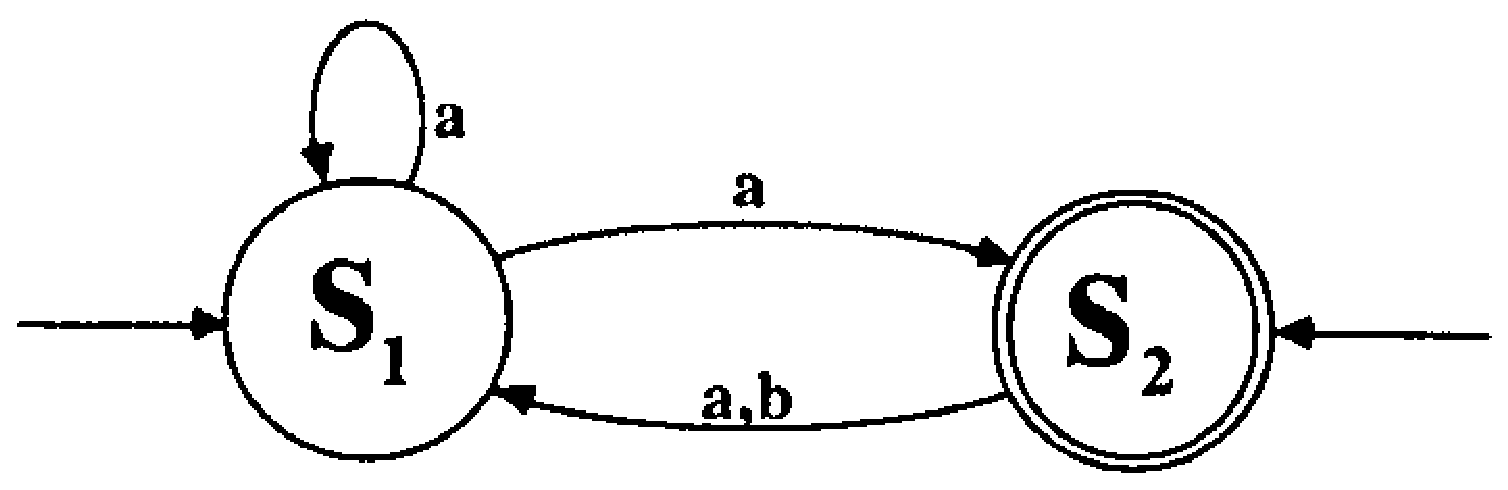
\epsfig{figure=ToFAfigures/fig6-11.eps,width=2.5in}}
\caption{The NDFA for Exercise 6.40}\label{fig-6.11}
\end{figure}
\item Solve these equations for both unknowns.
\item Give a regular expression that corresponds to the language accepted by
this NDFA.
\item Rework the problem with two left-linear equations.
\end{enumerate}

\item \begin{enumerate}
\item Use Theorem \ref{thm-6.3} to write the four right-linear equations in four unknowns
corresponding to the NDFA given in Figure \ref{fig-6.12}.
% Figure 6.12
\begin{figure}
\centerline{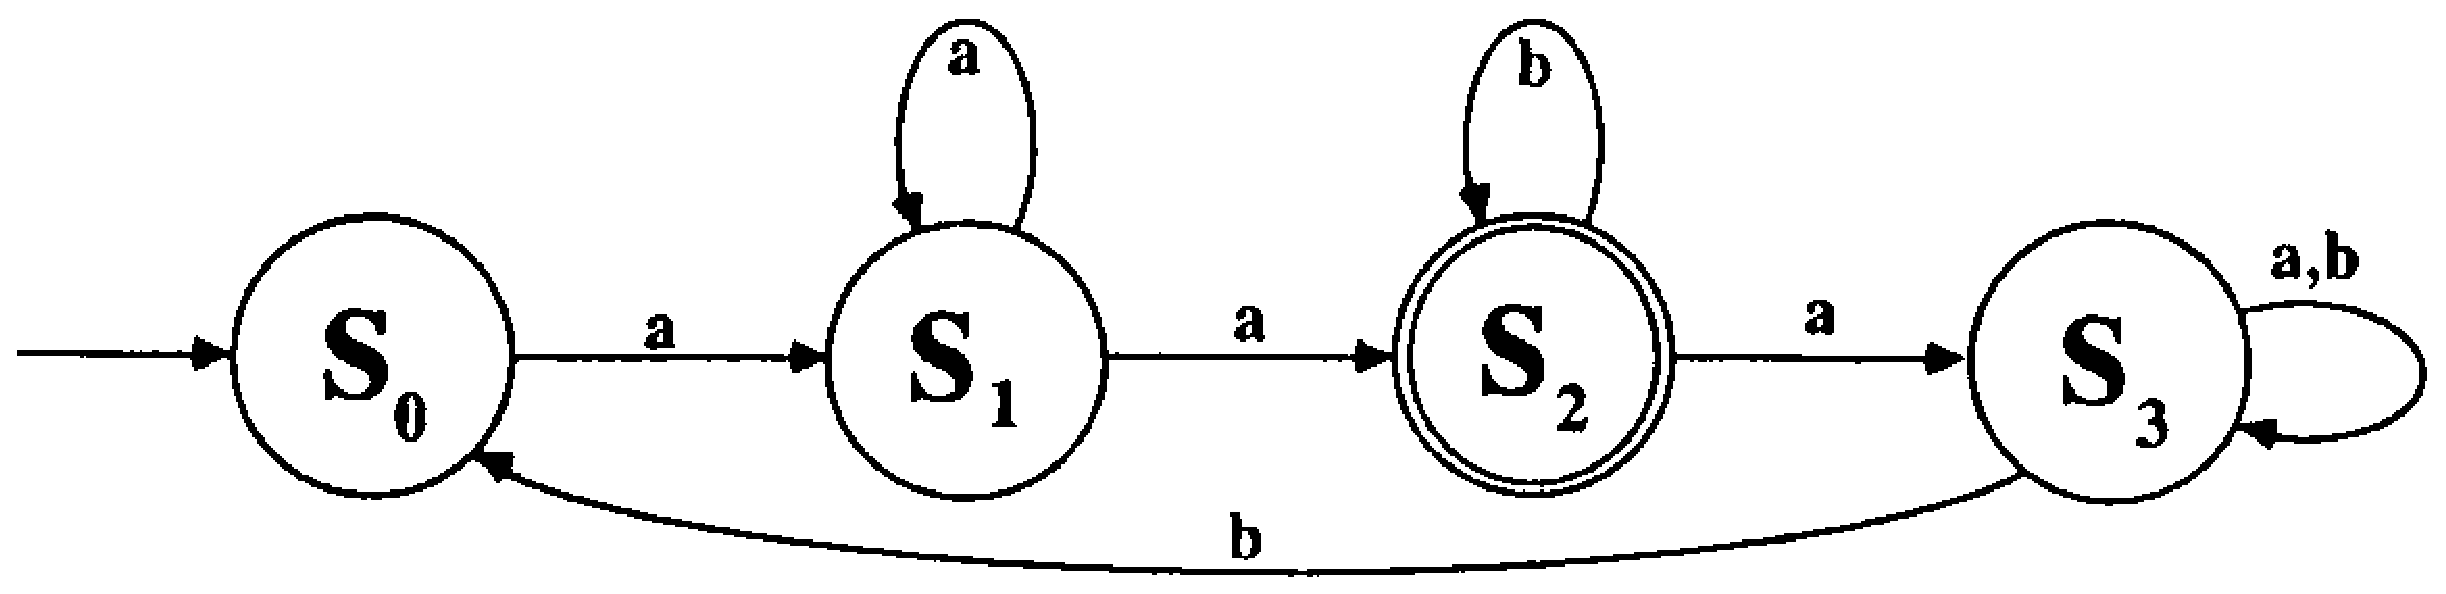
\epsfig{figure=ToFAfigures/fig6-12.eps,width=4.5in}}
\caption{The automaton for Exercise 6.41}\label{fig-6.12}
\end{figure}
\item Solve these equations for all four unknowns.
\item Give a regular expression that corresponds to the language accepted by
this NDFA.
\item Rework the problem with four left-linear equations.
\end{enumerate}

\item \begin{enumerate}
\item Use Theorem \ref{thm-6.3} to write the seven right-linear equations in seven
unknowns corresponding to the NDFA given in Figure \ref{fig-6.13}.
% Figure 6.13
\begin{figure}
\centerline{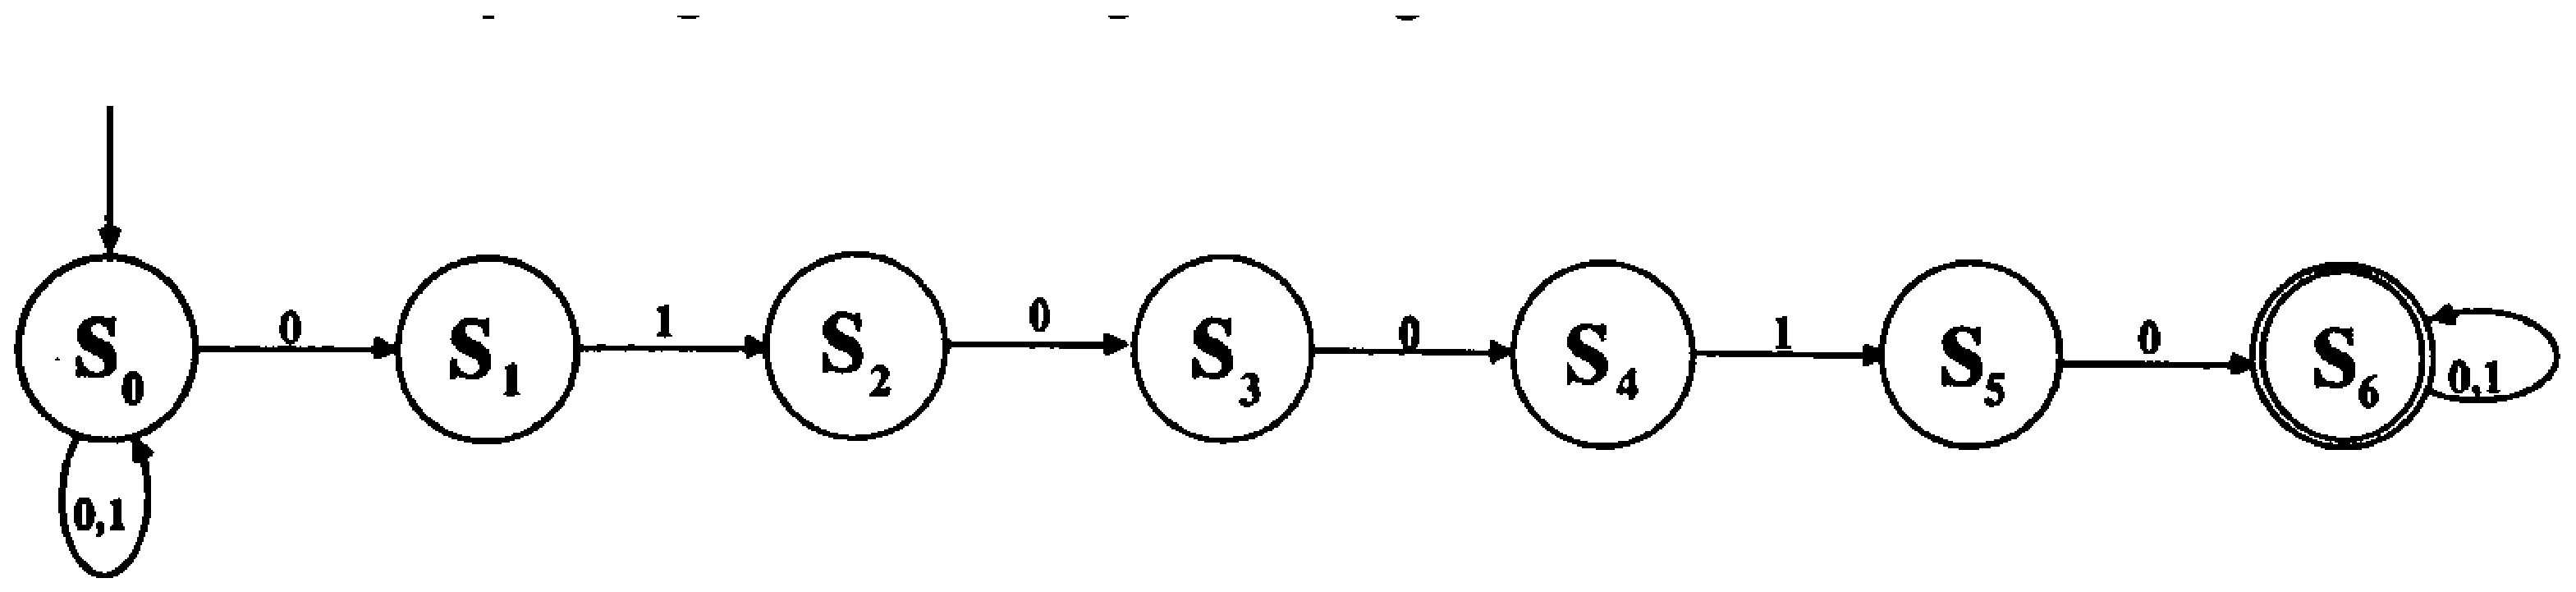
\epsfig{figure=ToFAfigures/fig6-13.eps,width=6.5in}}
\caption{The NDFA for Exercise 6.42}\label{fig-6.13}
\end{figure}
\item Solve these equations for all seven unknowns. \emph{Hint:} Make use of the
simple nature of these equations to eliminate variables without appealing to
Theorem \ref{thm-6.2}.
\item Give a regular expression that corresponds to the language accepted by
this NDFA.
\item Rework the problem with seven left-linear equations.
\end{enumerate}

\item Prove that for \emph{any} languages $A$, $E$, and $Y$, if $E \subseteq Y$,
then $A \cdot E \subseteq A \cdot Y$.

\item Let $\Sigma$ be an alphabet, and let $s:\ \Sigma \rightarrow \Gamma^*$ be
a substitution.
\begin{enumerate}
\item Prove that the image of \RSIG\ under $\overline{s}$ is contained in $\mathfrak{R}_{\Gamma}$.
\item Give an example to show that the image of \NSIG under $\overline{s}$ need
not be completely contained in $\mathfrak{N}_{\Gamma}$.
\end{enumerate}

\item Give a detailed proof of Lemma \ref{lmm-6.3}.

\item Let $\Sigma=\{\pmb{a},\pmb{b}\}$ and $\Xi=\{x \in \Sigma^*|\ x$ contains (at
least) two consecutive $\pmb{b}$s $\wedge x$ does \emph{not} contain two
consecutive $\pmb{a}$s$\}$. %Draw a machine that will accept $\Xi$.
Give a regular expression that describes this language.

\item Let $\Sigma = \{\pmb{a},\pmb{b},\pmb{c}\}$. Give regular expressions that will describe:
\begin{enumerate}
\item $\{x \in \{\pmb{a},\pmb{b},\pmb{c}\}^*\ |$ every $\pmb{b}$ in $x$ is eventually
followed by $\pmb{c}\}$; that is, $x$ might look like $\pmb{baabacaa}$, or
$\pmb{bcacc}$, and so on.
\item $\{x \in\{\pmb{a},\pmb{b},\pmb{c}\}^*\ |$ every $\pmb{b}$ in $x$ is immediately
followed by $\pmb{c}\}$.
\end{enumerate}

\item Let $\Sigma=\{\pmb{a},\pmb{b}\}$. Give, if possible, regular expressions
that will describe each of the following languages. Try to write these directly
from the descriptions (that is, avoid relying on the nature of the corresponding
automata).
\begin{enumerate}
\item The language consisting of all words that have neither consecutive
$\pmb{a}$s nor consecutive $\pmb{b}$s.
\item The language consisting of all words that begin and end with different
letters.
\item The language consisting of all words for which the last two letters match.
\item The language consisting of all words for which the first two letters
match.
\item The language consisting of all words for which the first and last letters
match.
\end{enumerate}

\item The set of all valid regular \emph{expressions} over $\{\pmb{a},\pmb{b}\}$
is a language over the alphabet $\{\pmb{a},\pmb{b},(,),\cup,\pmb{\cdot},^*,\emptyset,
\epsilon\}$. Show that this language is not FAD.

\item Give regular expressions corresponding to the languages accepted by each
of the NDFAs listed in Figure \ref{fig-6.14}.

\item Complete the details of the proof of Theorem \ref{thm-6.6}.

\item Prove Lemma \ref{lmm-6.4}.

\item Corollary \ref{cor-6.3} followed immediately from Theorem \ref{thm-6.6}. Show that Theorems
\ref{thm-5.2}, \ref{thm-5.4}, and \ref{thm-5.5} are also corollaries of Theorem
\ref{thm-6.6}.

% Figure 6.14
\begin{figure}
\centerline{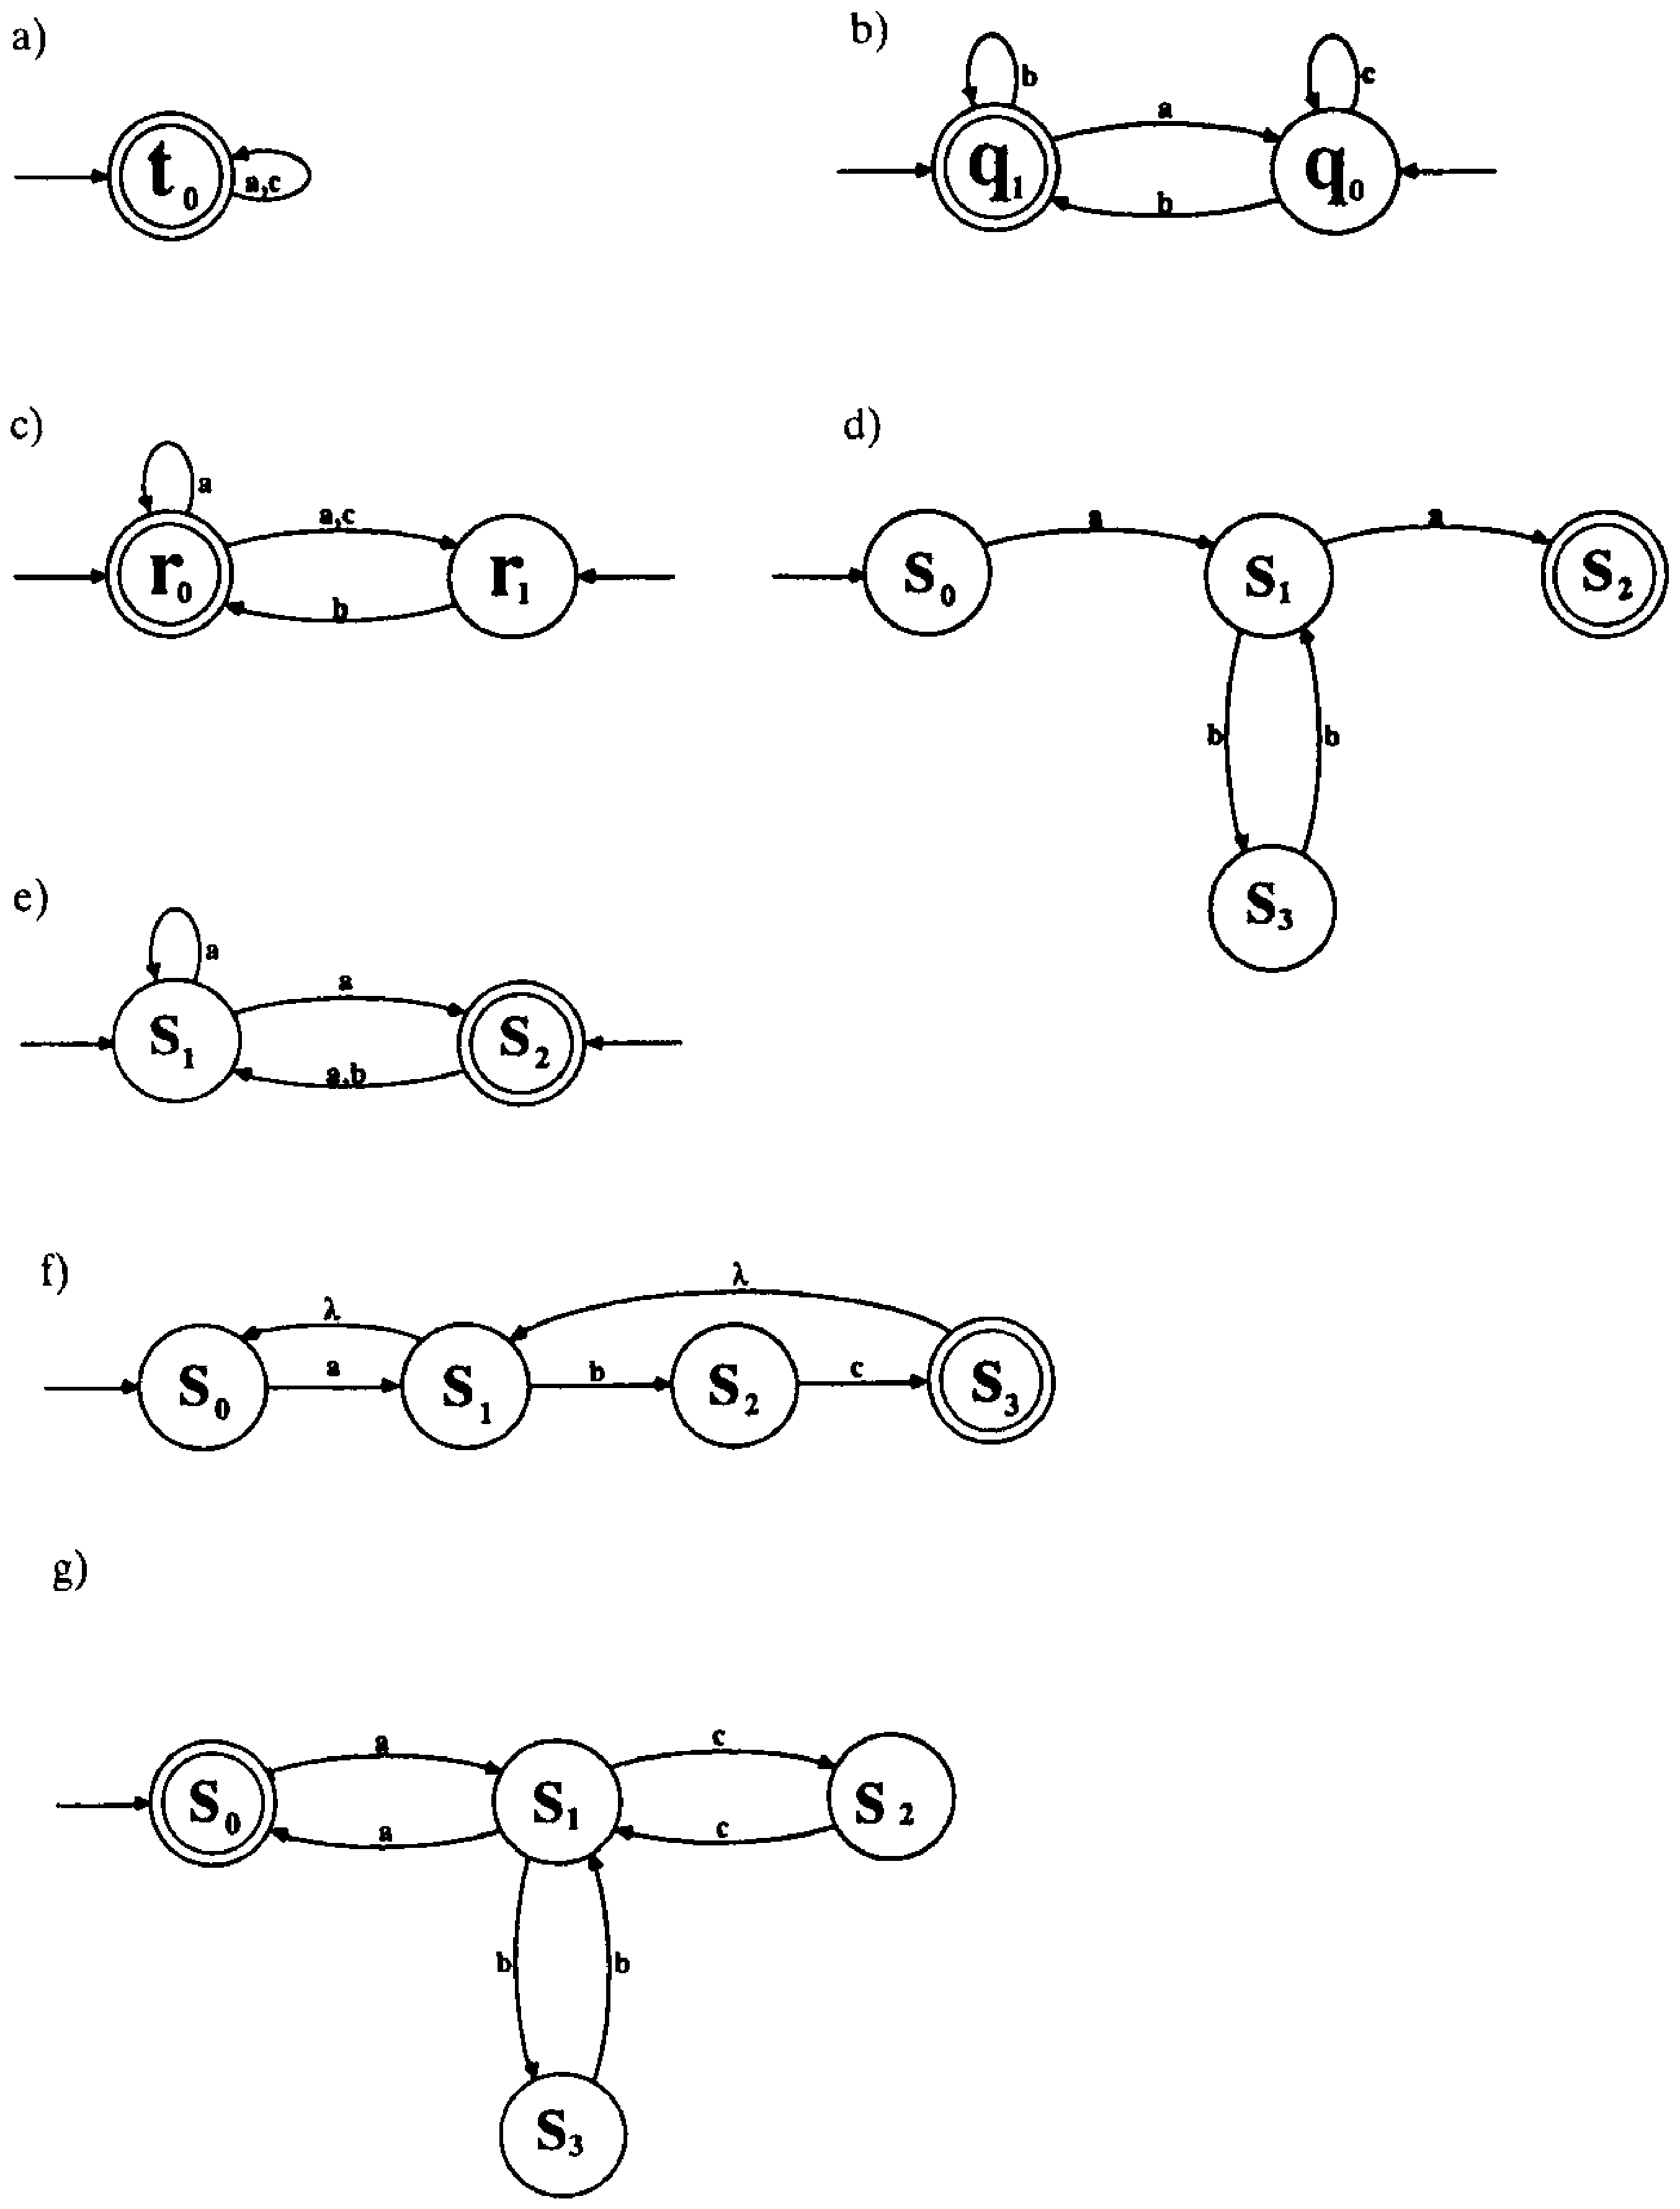
\epsfig{figure=ToFAfigures/fig6-14.eps,width=6.2in}}
\caption{The automata for Exercise 6.50}\label{fig-6.14}
\end{figure}

\item Let $\pmb{F}$ be the collection of languages that can be formed by repeated
application of the following five rules:
\begin{enumerate}[i.]
\item $\{\pmb{a}\}\in \pmb{F}$ and $\{\pmb{b}\}\in \pmb{F}$
\item $\{\ \}\in \pmb{F}$
\item $\{\lambda\}\in \pmb{F}$
\item If $F_1\in \pmb{F}$ and $F_2 \in \pmb{F}$, then $F_1 \cdot F_2 \in \pmb{F}$
\item If $F_1 \in \pmb{F}$ and $F_2 \in \pmb{F}$, then $F_1 \cup F_2 \in \pmb{F}$
\end{enumerate}
Describe the class of languages generated by these five rules.
\end{enumerate}
